\documentclass[11pt,a4paper]{report}
\usepackage[utf8]{inputenc}
\usepackage[english,portuges]{babel}
\usepackage{amsmath}
\usepackage{graphicx}
\usepackage{tabularx}
\usepackage{adjustbox}
%\usepackage[colorinlistoftodos]{todonotes}
\usepackage{csquotes}
\usepackage{comment}
\usepackage{imakeidx}
%tabela
\usepackage{multirow}
\usepackage{xcolor}
\usepackage[margin=3cm]{geometry}
\usepackage[hidelinks]{hyperref}
\usepackage[toc,acronym,nopostdot,nonumberlist]{glossaries}
\usepackage{titling}
\usepackage{tikzpagenodes}
\usepackage[ddmmyyyy]{datetime}
\usepackage{setspace}
\usepackage{indentfirst}
\usepackage[toc,page]{appendix}
\usepackage{tcolorbox}

\usepackage[table]{xcolor}
\usepackage{array}
\renewcommand{\arraystretch}{1.5} %altura da celula

\usepackage{float}

\usepackage[bottom]{footmisc}
%\usepackage{caption}
\usepackage{enumitem}
\usepackage{pgfgantt}
\usepackage{fancyhdr}
\usepackage{lastpage}
\usepackage{listings}
\usepackage{etoolbox}

\setlength {\marginparwidth }{2cm}
\usepackage[colorinlistoftodos,prependcaption,textsize=footnotesize]{todonotes}
% TODO PT: confirmar se isto é preciso \interfootnotelinepenalty=10000
%para definir a localização das tabelas e imagens em modo strict
%\usepackage{placeins}
\setcounter{tocdepth}{4}
\setcounter{secnumdepth}{4}

% ========================================
% PT: personalizações
\usepackage{url}
\usepackage{pdflscape}
\usepackage{rotating}
\usepackage{numprint}

% PT: ordenação das referências
\usepackage[sorting=none]{biblatex}

% PT: formatação das legendas das imagens
\usepackage{caption}
\captionsetup[figure]{labelfont={bf,scriptsize},textfont={scriptsize,it}}
\captionsetup[table]{labelfont={bf,scriptsize},textfont={scriptsize,it}}
\captionsetup[lstlisting]{labelfont={bf,scriptsize},textfont={scriptsize}}
\renewcommand{\lstlistingname}{Excerto}

\newcommand{\source}[1]{\vspace{-6pt}\caption*{\emph{(Fonte: {#1})}}}
\newcommand{\adaptedfrom}[1]{\vspace{-6pt}\caption*{\emph{(Adaptado de {#1})} }}


%-----------------------------------------------------------

\lstset{
   language=csh,
   backgroundcolor=\color{lightgray},
   extendedchars=true,
   basicstyle=\footnotesize\ttfamily,
   showstringspaces=false,
   showspaces=false,
   numbers=left,
   numberstyle=\footnotesize,
   numbersep=9pt,
   tabsize=2,
   breaklines=true,
   showtabs=false,
   captionpos=b
}


\lstset{
   language=Python,
   backgroundcolor=\color{lightgray},
   extendedchars=true,
   basicstyle=\footnotesize\ttfamily,
   showstringspaces=false,
   showspaces=false,
   numbers=left,
   numberstyle=\footnotesize,
   numbersep=9pt,
   tabsize=2,
   breaklines=true,
   showtabs=false,
   captionpos=b
}

\lstset{
   language=Bash,
   backgroundcolor=\color{lightgray},
   extendedchars=true,
   basicstyle=\footnotesize\ttfamily,
   showstringspaces=false,
   showspaces=false,
   numbers=left,
   numberstyle=\footnotesize,
   numbersep=9pt,
   tabsize=2,
   breaklines=true,
   showtabs=false,
   captionpos=b
}
%------------------------------------------------------------


% PT: caracteres
\usepackage{pifont}
\usepackage{newunicodechar}
\newunicodechar{✔}{\ding{51}}
%\DeclareUnicodeCharacter{2713}{✔}

\addbibresource{Z0-ref.bib}
%PT: eis alguns exemplos de como se inserem entradas de siglas
\newacronym{api}{API}{\emph{Application Programming Interface}}
\newacronym{http}{HTTP}{\emph{Hypertext Transfer Protocol}}
\newacronym{https}{HTTPS}{\emph{Hypertext Transfer Protocol Secure}}
\newacronym{ieee}{IEEE}{\emph{Institute of Electrical and Electronics Engineers}}
\newacronym{ietf}{IETF}{\emph{Internet Engineering Task Force}}
\newacronym{ip}{IP}{\emph{Internet Protocol}}
\newacronym{json}{JSON}{\emph{JavaScript Object Notation}}
\newacronym{ldap}{LDAP}{\emph{Lightweight Directory Access Protocol}}
\newacronym{lxc}{LXC}{\emph{Linux Containers}}
\newacronym{lxd}{LXD}{\emph{Linux Hypervisor}}
\newacronym{nat}{NAT}{\emph{Network Address Translation}}
\newacronym{rest}{REST}{\emph{Representational State Transfer}}
\newacronym{rfc}{RFC}{\emph{Request For Comments}}
\newacronym{sdk}{SDK}{\emph{Software development kit}}
\newacronym{ssh}{SSH}{\emph{Secure Shell Protocol}}
\newacronym{tcp}{TCP}{\emph{Transmission Control Protocol}}
\newacronym{udp}{UDP}{\emph{User Datagram Protocol}} 
\newacronym{url}{URL}{\emph{Uniform Resource Locator}} 
\newacronym{vm}{VM}{\emph{Virtual Machine}}
\newacronym{wsl}{WSL}{\emph{Windows Subsystem for Linux}}

\makeglossaries

%colocar aqui variáveis que serão utilizadas no texto:
\newcommand\kbps{\text{\textit{k}bit/s}}

\newenvironment{rotatepage}%
    {\clearpage\pagebreak[4]\global\pdfpageattr\expandafter{\the\pdfpageattr/Rotate 90}}%
    {\clearpage\pagebreak[4]\global\pdfpageattr\expandafter{\the\pdfpageattr/Rotate 0}}%

\newcommand{\specialcell}[2][c]{%
  \begin{tabular}[#1]{@{}c@{}}#2\end{tabular}}

\newdateformat{daymonthyear}{\THEDAY\ de \monthname[\THEMONTH], \THEYEAR}
\onehalfspacing
\parskip=5pt plus 1pt

\hyphenation{ISMAI}
\hyphenation{IPMAIA}
\hyphenation{UMAIA}
\hyphenation{Redmine}
\hyphenation{Subversion}
\hyphenation{Maieutica}
\hyphenation{DevLab}
\hyphenation{Relab}
\hyphenation{COVID}

\begin{document}

\begin{titlepage}
\doublespacing

\begin{tikzpicture}[remember picture,overlay,shift={(current page.center)}]
\node[anchor=center,xshift=0cm,yshift=9cm]{
\includegraphics[scale=4]{figs/logo_ipmaia_small.png}};
\end{tikzpicture}

\centering
\vspace{5cm}
\huge Projeto Plugin para o Forge do IPMAIA\\
\vspace{1cm}
\large Plugin de controlo de portas de containers\\
\vspace{2cm}

\Large Nuno Cardoso\\Aluno A036785\\2023/2024\\
\vspace{2cm}
\large Orientação de\\
\large Cláudia Freitas\\
\vspace{1cm}
\normalsize Tecnologias de Informação, Web e Multimédia\\do\\
Instituto Politécnico da Maia\\
\vspace{1cm}
Maia, \daymonthyear\today \\
\vspace{1cm}
%\includegraphics[scale=0.4]{figs/x.png}
%December, 2019
%\large v2.3
\end{titlepage}

\pagenumbering{roman}
\label{ficha}

Aqui deve ser colocada a ficha de caracterização.
\begin{abstract}
\label{resumo}

Este relatório descreve a descrição da elaboraboração de uma extensão de controlo
de portas TCP/UDP de \textit{containers} que poderá ser integrada na plataforma 
Forge (DevLab do IPMAIA/UMAIA).
Os principais vantagens desta extensão consistem aumentar a segurança através do 
controlo de serviços que são 
disponiblizados pelos \textit{containers}, facilitar as ações do administrador do 
sistema que envolvem o controlo de portas através de uma interface web.
\\
\\
\\
\textbf{Expressões-chave:} Extensão. Controlo de portas TCP/UDP. \textit{Containers}. Segurança.

\end{abstract}

\selectlanguage{english}

\begin{abstract}
\label{abstract}
This report describes the development of an plugin for controlling TCP/UDP 
ports of containers that can be integrated into the Forge platform (DevLab of 
IPMAIA/UMAIA). The main advantages of this extension are increasing security by 
controlling the services provided by the containers, and facilitating the system 
administrator's tasks involving port control through a web interface.
 \\
 \\
 \\
 \textbf{Key-expressions:} \textit{Plugin. Controlling TCP/UDP ports. Containers. Security.}
 
 
\end{abstract}
\selectlanguage{portuges}


% PT: Toda esta secção é facultativa
\chapter*{Declaração de honra}
\label{way_of_the_samurai}
Por este meio se declara que este documento é conteúdo original, produzido pelo identificado como autor, não tendo sido previamente apresentado noutro percurso académico ou unidade curricular de qualquer instituição.

Quaisquer referências a outros trabalhos respeitam rigorosamente os regulamentos e melhores práticas de
atribuição, sendo apropriadamente marcadas no texto e identificadas na secção \emph{\nameref{chapter:refs}} na página \pageref{chapter:refs}, sob as normas \acrshort{ieee}\footnote{\acrshort{ieee} --- \acrlong{ieee}} de referenciação.

O autor igualmente declara não se encontrar em qualquer situação de conflito de interesses efectiva ou potencial, por não haver qualquer envolvimento com elementos passíveis de selecção.

%\nameref{chapter:refs}

% TODO PT: reescrever tudo
\chapter*{Agradecimentos}

Aqui, se assim for intenção do autor, se deverá colocar o texto com os agradecimentos. % PT: este capítulo é opcional
%insert index
\tableofcontents

\phantomsection
\addcontentsline{toc}{chapter}{\listtablename} % PT: lista de tabelas. Não modificar
\listoftables

\phantomsection
\addcontentsline{toc}{chapter}{\listfigurename}	% PT: lista de figuras. Não modificar
\listoffigures

\phantomsection
\renewcommand{\lstlistlistingname}{Lista de excertos de código e terminal}
\addcontentsline{toc}{chapter}{\lstlistlistingname}	% The List of Figures (Do not modify)
\lstlistoflistings
\glsaddall
\printglossary[type=\acronymtype]
\printglossary[type=main,title={Glossário},toctitle={Glossário}]
\pagenumbering{arabic}

\chapter{Introdução}
\label{chap:introduction}

Este relatório pretende demonstrar o trabalho realizado para este projeto.
O mesmo consiste num mecanismo de controlo de portas TCP/UDP \cite{rfc9293},
\cite{rfc768} dos \textit{containers} ou do próprio sistema \textit{host}
da plataforma Forge do IPMAIA.

Esta extensão à plataforma Forge, tem 
como principal objetivo de facilitar a gestão as conexões \textit{containers} 
que são disponibilizados, fazendo uso de ima interface \textit{web}, onde o adminitrador da 
plataforma pode receber pedidos para abrir novas conexões. 

Para a concretização deste trabalho são necessários os seguintes objetivos:\\

\begin{itemize}
\item \textit{Daemon} que irá interagir com a \textit{firewall} ou \acrshort{api}\footnote{\acrshort{api} -- \acrlong{api}} do sistema de \textit{containers};
\item Interface \textit{Web} e \acrshort{api} para interagir com o Daemon;
\item Sistema de notificações de eventos para Microsoft Teams, Discord e E-mail.
\end{itemize}


\section{Objetivos}
\label{sec:object}

Pretende-se, com este projecto, acrescentar funcionalidades/facilitar tarefas na plataforma ao
DevLab/Forge do IPMAIA/UMAIA que permitam:

\begin{itemize}
\item o administrador do sistema facilmente defenir regras de \textit{firewall} no sistema host da plataforma (através do terminal ou de uma interface web);
\item a atribuíção de endereços \acrshort{ip}\footnote{\acrshort{ip} -- \acrlong{ip}} a \textit{containers} hospedados na plataforma, de modo,
a dar conectividade aos mesmos (através do terminal ou de uma interface web);
\item controlar quais portas dos \textit{containers} são disponiibilizadas para a rede interna da intituição;
\item os alunos, aos quais, lhes foram atribuídos um \textit{container}, fazer um pedido ao administrador do sistema para poder
obter ou não conectividade em determinada porta \acrshort{tcp}/\acrshort{udp};
\item os alunos que efetuaram um pedido de abertura de porta, receber notificação (por Microsoft Teams, Discord ou E-mail) quando O
pedido for aceite ou negado.

\end{itemize}

Com a enumeração dos objetivos referidos, serão demonstrados ao longo deste documento
todo o proceso de desnvolvimentos dos mesmos.




\section{Metodologia}
\label{sec:intro_method}

A metodologia usada neste projeto começa com o desenvolvimento base do "Port Controller",
da Rest API e da unix socket que permite aos dois comunicarem. Após ter essa base funcional
foi realizada uma pesquisa sobre Iptables, Nftables, LXC e LXD e de como interagir estes, tanto
por linha de comandos como através de código C\#. Foi feita também uma pesquisa de como
outras plataformas abordam o tópico de controlo de conexões de \textit{containers}.
Por consequente, deu-se continuidade ao desenvolvimento do "Port Controller" e dos 
restantes componentes e à realização de testes dos mesmos.


\section{Recursos tecnológicos}
\label{sec:intro_resources}


No que diz respeito a recursos tecnológicos, optou-se por usar as seguintes opções:

\begin{itemize}
\item Linguagem C\# com o \textit{framework .NET Core} 7.0 para a criacção do \textit{daemon} que gere
as portas dos \textit{containers} e \textit{unix socket de servidor};
\item Linguagem Python versão 3.11 a \textit{unix socket} cliente;
\item Linguagem Python versão 3.11 com a biblioteca Flask para a API e sistemas de notificações;
\item Linguagem Python versão 3.11 com a biblioteca Flask interface \textit{Web}, juntamente com \acrshort{html}\footnote{\acrshort{html} -- \acrlong{html}}, \acrshort{css}\footnote{\acrshort{css} -- \acrlong{css}}, Javascipt e Bootstrap.
\item Máquina virtual com alpine linux 3.19 e \acrshort{wsl}\footnote{\acrshort{wsl} -- \acrlong{wsl}} com ubuntu 22.04 para testar o projeto.
\end{itemize}




\section{Cronograma}
\label{sec:intro_chronos}

\begin{figure}[H]
\begin{center}
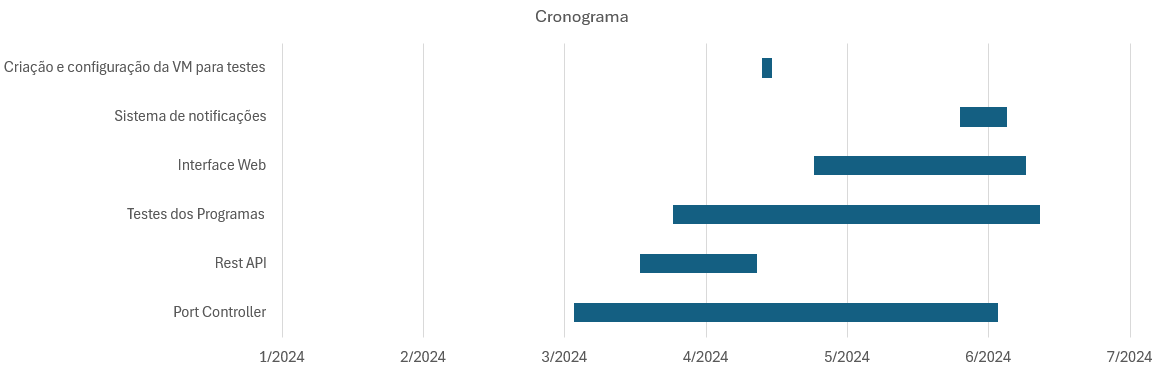
\includegraphics[width=16cm]{figs/cronograma.png}
\caption{Cronograma do projeto}
\label{fig:bookstack}
\end{center}
\end{figure}


\section{Organização do relatório}
\label{sec:intro_struct}

Este documento está organizado pelos seguintes tópicos:

Este relatório está organizado e vários capítulos, de modo, a explicar de forma
eficaz todo o processo no decorrer da elaboração deste projeto.

O documento inicia-se com o Resumo em língua Portuguesa e o Resumo em língua 
inglesa (Abstract), seguindo-se a Declaração de honra e dos Agradecimentos.

O capítulo 1, Introdução, apresenta o tema do projeto realizado, mencionado tópicos
como os Objetivos e Recursos tecnológicos.

No capítulo 2, Análise do problema, é explicado os problemas que este projeto 
pretende resolver.

No capítulo 3, Fundamentos teóricos, são referidos tecnologias e conceitos relevantes 
para o desenvolvimento do projeto, nela são mencionadas as linguagens de programação usadas,
programas utilizados e funcionamento destes.

O capítulo 4, Estado da Arte, dá exemplos do funcionamento das conexões de outras 
plataformas, tais como Google Cloud e Microsoft Azure.

No capítulo 5, Desenvolvimento do tema, onde é abordado as configurações do sistema
de testes, testes do iptables e LXD e desenvolvimento do código dos componentes 
do projeto.


No capítulo 6, Desvios de procedimento, fala sobre pontos que se desviaram do planeamento inicial.

Segue-se o capítulo 7, para apresentar a Discussão de resultados.

No capítulo 8, Trabalho futuro, são referidas possiveis melhoramentos ou adição de funcionalidades
do projeto.

Por fim, no capítulo 9, apresenta-se as Conclusões e a reflexão crítica.


\section*{Sumário}
\label{sec:intro_summary}
%Se considerar relevante, faça um pequeno resumo do capítulo. É uma secção opcional que pode ser eliminada, mas altamente recomendada.
Considera-se assim haver uma possibilidade de aumentar a segurança e controlo do que é disponibilizado
pelos \textit{containers} atribuídos aos alunos.
\\
\\
%Abaixo deve usar a instrução {\textbackslash}cite\{\} para colocar uma relação das citações utilizadas no texto deste capítulo. Aqui liste apenas as citações, pela ordem em que aparecem no texto -- não coloque mais texto. Exemplo:
\\
\\
%\textbf{Referências relevantes:}  \cite{ismai_ead}, \cite{rfc4512}.
\chapter{Análise do problema}
\label{cap:problem}

Descrever aqui o problema que se pretende resolver.


Olha que giro, uma lista:

\begin{enumerate}
    \item item1;
    \item item2;
    \item item3;
    \item item4.
\end{enumerate}


E uma lista não numerada... nice;

\begin{itemize}
    \item abc;
    \item def.
\end{itemize}

O Forge da Universidade da Maia e IPMaia é um serviço com multiplas funções com 
o objetivo de ajudar os alunos a desenvolver os seus trabalhos.
Uma das suas funções é a disponibilização de \textit{containers} que podem ser usados
para alojar aplicações/programas desenvolvidos pelos alunos.

Estes \textit{containers} que são disponibilizados por norma precisam de 
abrir/fechar portas TCP/UDP para o funcionamento de programas ou para os
utilizadores interagirem com o mesmo, como por exemplo a porta 22 usada para o 
SSH \cite{rfc4253}.

Atualmente, não existe um sistema se controlo de portas ou \textit{firewall}, neste momento qualquer container
consegue abrir portas e deixá-las acessiveis para qualquer utilizador dentro da rede local
do IPMAIA/UMAIA.

Sendo assim seria útil haver uma método mais fácil e cómodo para o administrador do sistema
controlar e decidir que portas os \textit{containers} do utilizadores deverão expor para a rede local.



\section*{Sumário}

Idem... 

% PT: opcional
\chapter{Fundamentos teóricos}
\label{chap:theo}

Este capítulo é opcional \textbf{mas altamente recomendado} e, a existir, deve descrever os Fundamentos Teóricos, o que incluirá descrever as tecnologias relevantes, sejam concorrentes ou de fundação.

Neste capitulo serão abordadas tecnologias e fundamentos teóricos relevantes para 
este projeto. \\

\section{Distribuições Linux}

Sendo Linux apenas um \textit{Kernel}, ou seja, um "nucleo" de um sistema operativo
o mesmo não pode ser usado si só da mesma forma que outros sistemas operativos.
Para ter um sistema completo é necessário adicionar multiplos programas/bibliotecas,
sendo assim, existe um numero elevado de sistemas operativos basedos em Linux.

Certas distribuições podem ter diferentes alvos de utilizadores/utilização, quer seja,
para uso pessoal/tradicional de um utilizar comum, quer seja para servidores.

As principais vantagens associadas ao uso de um Sistema operativo baseado em Linux são:
\begin{enumerate}
    \item Não é preciso licensa de utilização;
    \item Código aberto;
    \item É um sistema que por norma consome menos recursos que a maioria das distribuições disponiveis;
    \item costumização.
\end{enumerate} 



\section{Alpine Linux}

"Alpine Linux é uma distribuição Linux baseada em musl e BusyBox originalmente
projetada para utilizadores avançados que apreciam segurança, simplicidade e eficiência 
no uso de recursos." \cite{alpinewiki}

O Alpine Linux é uma distribuição independente, isto é, não baseda em nunhuma 
outra distribuição como muitas outras. E usada principalmente em ambientes
profissionais/servidores.

Esta distribuição é projetada para ser extremamente leve, com uma instalação 
mínima que ocupa apenas alguns megabytes de espaço. \\

\subsection{Segurança do sistema}

É também focada em ser um sistema 
seguro daí incorporar  medidas como o \textit{Position Independent Executables} (PIE) e 
o \textit{Stack Smashing Protection} (SSP) por padrão.

O \textit{Position Independent Executables} (PIE) são um tipo de executável que pode ser 
carregado em qualquer endereço da memória, ao contrário de executáveis tradicionais 
que são carregados para um endereço fixo. Isto aumenta a segurança do sistema uma vez que
o PIE usa o ASLR (\textit{Address space layout randomization}) para criar aleatoriedade
nas posições de áreas-chave de memória, como a \textit{stack}, o heap e as bibliotecas compartilhadas.

Desta forma com os executáveis sendo carregados em diferentes endereços em cada execução, 
é muito mais difícil para os atacantes desenvolverem explorações confiáveis que funcionem 
em todas as execuções.


O \textit{Stack Smashing Protection} (SSP) é uma técnica de segurança usada para detectar e
prevenir ataques de \textit{buffer overflow}. Este método consiste no SSP introduzir um valor 
especial conhecido como "\textit{canary}" entre a \textit{stack} de variáveis locais e o endereço de 
retorno da função. Antes de uma função retornar, o valor do "\textit{canary}" é verificado.
Se o "\textit{canary}" tiver sido alterado (indicando assim que a \textit{stack} foi corrompida), 
o programa é abortado. 

Para garantir estas técnicas de segurança no sistema, todos os pacotes no Alpine Linux
são compilados com suporte a PIE, garantindo que todos os executáveis possam se 
beneficiar da ASLR.

O compilador tem que ser também configurado para incluir proteção SSP por padrão,
adicionando "\textit{canarys}" de \textit{stack} aos binários compilados para detectar 
e mitigar \textit{buffer overflows}.



\subsection{Diferenças entre o Alpine Linux em relação a outras distribuições}

Principais diferenças do Alpine Linux com a maioria das distribuições Linux disponiveis são:
\begin{itemize}
    \item O seu \textit{init system} é o OpenRC;
    \item A \textit{shell} predefenida é o busybox ao contrário do famoso \textit{Bash} ou ZSH;
    \item Gestor de pagotes é o "\texttt{apk} (\textit{Alpine Package Keeper})";
    \item Por padrão, para executar comandos de forma administrativa é ncessário usar do comados "\texttt{doas}" em vez do "\texttt{sudo}".
\end{itemize} 

\subsection{Conlusão}

Em suma, o Alpine Linux é uma excelente escolha quando o objetivo é ter um sistema 
leve, seguro e eficiente, especialmente adequado para ambientes de servidores, containers
e sistemas embutidos.


\section{Linguagens de programação}

Nesta secção serão abordadas liguagens de programação relevantes no projeto.

\subsection{Linguagem C\# (.NET Core)}

O C\# (C Sharp) é uma linguagem de programação desenvolvida pela Microsoft e é amplamente
utilizada para desenvolver aplicações para a plataforma .NET. A versão .NET Core 
é uma implementação de código aberto, multiplataforma e modular do .NET,
que suporta o desenvolvimento de aplicações utilizando C\#.

As principais carecterias do o \textit{framework} .Net Core são:

\begin{itemize}
\item \textbf{Multiplataforma}:  .NET Core é projetado para ser executado em diversas 
plataformas, incluindo Windows, macOS e Linux. Isso permite que os desenvolvedores criem 
aplicações .NET que podem ser executadas nos principais sistemas operativos;
\item \textbf{Código Aberto}: Tanto o .NET Core quanto o C\# são projetos de código
aberto hospedados no GitHub. Isso significa que os desenvolvedores podem contribuir
com melhorias, correções de bugs e novos recursos para a linguagem e framework;
\item \textbf{Desempenho}:  .NET Core foi otimizado para oferecer um melhor desempenho
em comparação com as versões anteriores do .NET Framework. 
Isso inclui melhorias no tempo de inicialização, uso de memória e desempenho de execução;
\item \textbf{Compatibilidade com o Ecossistema .NET}: Embora o .NET Core seja uma 
implementação mais leve e focada do .NET, ele ainda é compatível com grande parte
do ecossistema .NET existente. Isto significa que os desenvolvedores podem aproveitar
bibliotecas e ferramentas existentes ao desenvolver aplicações com .NET Core e C\#;
\item \textbf{Suporte a Tecnologias Modernas}:O .NET Core suporta características 
modernas da linguagem C\#, como \texttt{async/await} para programação assíncrona, padrões de 
programação funcional e muito mais. Isto permite que os pra quem desenvolve aproveite as 
melhores práticas de desenvolvimento de software ao escrever código em C\# para .NET Core.
\end{itemize}


As principais carecterias da linguagem C\# são:


\begin{itemize}
\item \textbf{Tipagem Estática}: C\# é uma linguagem de tipagem estática, o que 
significa que o tipo de cada variável é determinado em tempo de compilação e deve 
ser declarado explicitamente;

\item \textbf{Orientação a Objetos}: C\# é uma linguagem orientada a objetos, 
onde os conceitos de classes e objetos são fundamentais. Tem suporte a heranças, 
encapsulamento, polimorfismo e outras características típicas da programação 
orientada a objetos;

\item \textbf{Sintaxe Simples e Legível}: A sintaxe de C\# é projetada para 
ser fácil de ler e entender. Isto é facilitado pelo uso de palavras-chave intuitivas 
e pela estrutura clara do código;

\item \textbf{Coleta Automática de Lixo (Garbage Collection)}: C\# possui um sistema 
de coleta automática de lixo que faz a gestão da alocação e libertação de memória, 
permitindo que os desenvolvedores se concentrem na lógica do programa sem se preocupar
com bugs relacionados à memória;

\item \textbf{Segurança de Tipo}: C\# é uma linguagem fortemente tipada, o que 
significa que o compilador verifica os tipos em tempo de compilação, ajudando a evitar 
erros comuns relacionados à manipulação de dados;


\item \textbf{Biblioteca Padrão Abrangente}: C\# é acompanhado por uma ampla 
biblioteca padrão, conhecida como .NET \textit{Framework} (ou .NET Core), que oferece
suporte a uma variedade de funcionalidades, como manipulação de ficheiros, acesso a bases 
de dados, desenvolvimento web, entre outros.
\end{itemize}



\subsection{Linguagem Python}


Python é uma linguagem de programação de alto nível, interpretada, dinâmica e 
multiparadigma. Ela foi criada por Guido van Rossum e lançada pela primeira vez em 1991.
Desde então, tornou-se uma das linguagens de programação mais populares do mundo devido
à sua simplicidade, legibilidade e versatilidade.

"Python é uma linguagem de programação de alto nível e propósito geral. A sua filosofia
de design enfatiza a legibilidade do código com o uso de indentação significativa.

Python é dinamicamente tipada e possui coleta de lixo automática. 
Suporta múltiplos paradigmas de programação, incluindo estruturada (particularmente 
procedural), orientada a objetos e programação funcional. É frequentemente descrita como 
uma linguagem "com tudo incluído", devido à sua biblioteca padrão abrangente." \cite{python}



As principais cracteriasaticas desta linguagem são:

\begin{itemize}
\item \textbf{Sintaxe Clara e Concisa}: Python é conhecido pela sua sintaxe limpa
e fácil de ler, o que a torna ideal para iniciantes e facilita a manutenção de código;
\item \textbf{Tipagem Dinâmica}: Em Python, não é necessário declarar explicitamente o
tipo de uma variável. O tipo é inferido dinamicamente durante a execução do programa;
\item \textbf{Multiparadigma}: Python suporta diversos paradigmas de programação,
incluindo programação orientada a objetos, programação imperativa e programação funcional;
\item \textbf{Biblioteca Padrão Abrangente}: Python vem com uma vasta biblioteca 
padrão que oferece suporte para uma ampla gama de tarefas, desde manipulação de arquivos 
até desenvolvimento web;
\item \textbf{Comunidade Ativa}:Python possui uma comunidade enorme e ativa de 
desenvolvedores em todo o mundo. Isto resulta numa grande quantidade
de recursos disponíveis, como bibliotecas de terceiros, frameworks e ferramentas 
de desenvolvimento.
\end{itemize}


"Python é suficientemente rápido para o nosso site e permite-nos produzir funcionalidades 
mantíveis em tempos recorde, com um mínimo de programadores." \cite{pyyt}


\section{Bibliotecas/FrameWorks relevantes para o projeto}

dfgs

\subsection{Flask (Python)}


dfgs

\section{APIs}

Nesta secção serão explicadas as APIs e como esta funcionam.


\subsection{O que é uma API?}

Uma API (Application Programming Interface) é uma interface que permite a interação entre diferentes componentes de software. 
Ela define métodos e protocolos de comunicação para que desenvolvedores possam utilizar 
funcionalidades específicas sem precisar entender os detalhes internos da implementação.
O serviço ao qual uma API pode estar associada pode ser um sistema operativo, uma biblioteca
de \textit{software} ou um serviço \textit{web}.

Alguns exemplos de APIs são a API do sistema de ficheiros do Node.js o "fs" e o DirectX 
da Microsoft, usada para tarefas relacionadas com multimídia e gráficos.

\subsection{O que é uma REST API?}


"A REST API (also called a RESTful API or RESTful web API) is an application 
programming interface (API) that conforms to the design principles of the representational
state transfer (REST) architectural style. REST APIs provide a flexible, lightweight way 
to integrate applications and to connect components in microservices architectures." \cite{ibmrestapi}



Uma REST API é um tipo de API que adere aos princípios do REST que é uma arquitetura
de \textit{software} orientada a serviços \textit{WEB}.
A lógica deste de funcionamento consiste em computadores enviarem recursos textuais através
de solicitações \textit{HTTP} pela \textit{internet} para um URL específico. \\

Alguns exemplos de REST APIs são a API do Discord que permite um utilizador mandar mensagens fora
da aplicação de cliente, usando apenas solicitações \textit{HTTP}, outra plataforma é 
o X (antigo Twitter) fazer "tweets" da mesma forma.


As solicitações \textit{HTTP} possuí as seguintes operações:
\begin{itemize}
    \item GET - Usado para solicitar dados de um recurso específico;
    \item HEAD - Similar ao GET, mas só retorna os cabeçalhos da resposta sem o corpo;
    \item POST - Enviar dados ao servidor para criar um novo recurso; 
    \item PUT - Atualizar um recurso específico com dados novos;
    \item PATCH - Atualizar parcialmente um recurso existente; 
    \item DELETE - Usado para apagar um recurso específico; 
    \item CONNECT - Principalmente usado para iniciar uma comunicação
    segura (via SSL/TLS) com um servidor proxy; 
    \item OPTIONS - Usado para descobrir os métodos suportados pelo servidor para um recurso específico;
    \item TRACE - Usado para depurar e rastrear o caminho que uma solicitação HTTP percorre.
\end{itemize}


Os principais formatos de texto a serem enviados nas solicitações são:
\begin{itemize}
    \item HTML;
    \item JSON;
    \item XML.
\end{itemize}


\section{Unix Socket}

Uma Unix Socket, também conhecida como Unix Domain Socket, 
é um mecanismo de comunicação interprocessual  que permite a troca de dados 
entre processos executados no mesmo sistema operativo.

Unix Sockets são frequentemente utilizados em sistemas Unix e Unix-like
(como Linux e macOS) para proporcionar uma comunicação eficiente e de baixa 
latência entre processos.


\subsection{Como funciona?}

Diferente das sockets de rede (TCP/IP), as Unix Sockets são usadas para 
comunicação local entre processos no mesmo sistema. Estas não dependem de interfaces 
de rede ou protocolos de rede.

Em vez de usar endereços IP e números de porta, as Unix Sockets utilizam caminhos 
no sistema de ficheiros (ex.: /tmp/socketfile).

\section{Containers}

\textit{Containers} são uma tecnologia de virtualização a nível de sistema operativo que 
permite executar várias aplicações ou sistemas operativos isolados em um único \textit{host}, usando o mesmo kernel. 
Fornecem ainda um ambiente leve, portátil e eficiente para empacotar e executar aplicações,
oferecendo isolamento semelhante ao das máquinas virtuais, mas com a uma menor
exigência de recursos.

Alguns exemplos de getores de \textit{containers} disponiveis atualmente:
\begin{itemize}
    \item Docker;
    \item LXD/LXC;
    \item rkt (Rocket);
    \item CRI-O;
    \item Podman.
\end{itemize}



\subsection{LXD e LXC}

LXD e LXC serão a principal tecnologia de \textit{containers} abordada neste projeto,
uma vez que é a mesma usada na plataforma Forge do IPMAIA/UMAIA. \\



\title*{\textbf{LXC (Linux Containers)}}

LXC é uma tecnologia de \textit{contaianers}, inicialmente desenvolvido pela IBM, 
de baixo nível que fornece containers leves e isolados usando namespaces e cgroups 
do kernel do Linux. \\

\begin{itemize}
    \item Namespaces: Proporcionam isolamento para processos, IDs de utilizadores, 
    sistema de ficheiros, redes, IPC (Inter-Process Communication), etc.;
    \item Cgroups: Gerem e limitam os recursos (CPU, memória, I/O) que um
    \textit{container} pode usar.
\end{itemize}

\title*{\textbf{LXD}}

Patrocinado pela Canonical Ltd. desde a sua  criação, LXD é uma camada de gestão para LXC, 
que oferece uma experiência de utilização mais amigável e recursos avançados.

As principais vantagens associadas ao LXD são:
\begin{itemize}
\item Interface de Linha de Comando (CLI): Comando "lxc" para gerir \textit{containers}
de maneira intuitiva;
\item API REST: Fornece uma API RESTful através de unix sockets ou solicitações HTTP para automação e integração com outras ferramentas.
\item \textit{Snapshots} e \textit{Backups}: Suporte para \textit{snapshots} e \textit{backups} dos \textit{containers}.
\item \textit{Live Migration}: Permite a migração ao vivo de \textit{containers} entre \textit{hosts}.
\item Uso de {Clusters}: Possibilidade de criar clusters de múltiplos hosts para gestão centralizada de \textit{containers}.
\end{itemize}


\subsection{Incus}

Incus é a próxima geração de gestão para LXC, com o princiapl objetivo de substituiur
O LXD.

\section{FireWalls Linux}

O \textit{kernel} Linux possui desde a versão 2.4, um \textit{framework} de filtragem de pacotes 
conhecido por Netfilter \cite{netfilter}. Este é utilizado utilizado para manipular e inspecionar 
pacotes de rede à medida que entram, saem ou atravessam o sistema.

Porem, a forma mais comum de interagir com o Netfilter é com outras ferramentas,
nomeadamente as duas mais conhecidas, o Iptables e o Nftables.

\subsection{Iptables}

O Iptables é a principal ferramenta associada ao Netfilter, que é uma interface
de linha de comando para configurar regras de filtragem de pacotes.
É posivel definir políticas de segurança, encaminhamento de pacotes,
redirecionamento de portas. 

As funcionalidades do Iptables são organizadas em \textit{tables} ou tabelas
sendo as principais as a \textit{Filter Table}, a \textit{Nat Table} e a
\textit{Mangle Table}, como se pode ver na tabela \ref{ipt1}.

\begin{table}[h]
\centering
\begin{tabular}{|c|c|c|}
\hline
\multicolumn{3}{|c|}{Iptables}\\
\hline
\rowcolor{yellow!50}\textbf{Filter Table} & \textbf{Nat Table} & \textbf{Mangle Table}\\
\hline
INPUT CHAIN & OUTPUT CHAIN & INPUT CHAIN\\
\hline
OUTPUT CHAIN & PREROUTING CHAIN & OUTPUT CHAIN\\
\hline
FORWARD CHAIN & POSTROUTING CHAIN & FORWARD CHAIN\\
\hline
- & - & PREROUTING CHAIN\\
\hline
- & - & POSTROUTING CHAIN\\
\hline
\end{tabular}
\caption{Tabelas principais do Iptables.}
\label{ipt1}
\end{table}


As principais funcionalidades de cada Table são:

\begin{itemize}
\item \textbf{\textit{Filter Table}}: Esta tabela é usada para filtrar pacotes com base em 
políticas de filtragem, como permitir, negar ou descartar pacotes;
\item \textbf{\textit{Nat Table}}: Esta tabela é usada para modificar endereços IP e portas
nos cabeçalhos dos pacotes, principalmente para implementar NAT;
\item \textbf{\textit{Mangle Table}}: Esta tabela é usada para alterar pacotes de maneiras
não abrangidas pelas outras tabelas. Isso pode incluir marcação de pacotes para fins especiais.
\end{itemize}



Existe ainda outras duas tabelas secundarias com propósitos mais simples, dadas 
por \textit{Raw Table} e \textit{Security Table}, como se pode ver na
tabela \ref{ipt2}.


\begin{table}[h]
\centering
\begin{tabular}{|c|c|}
\hline
\multicolumn{2}{|c|}{Iptables}\\
\hline
\rowcolor{yellow!50}\textbf{Raw Table} & \textbf{Security Table}\\
\hline
OUTPUT CHAIN & INPUT CHAIN \\
\hline
PREROUTING CHAIN & OUTPUT CHAIN \\
\hline
- & FORWARD CHAIN \\
\hline
\end{tabular}
\caption{Tabelas secundárias do Iptables.}
\label{ipt2}
\end{table}
    

\begin{itemize}
\item \textbf{\textit{Raw Table}}: Esta tabela é usada rastrear conexões, com um mecanismo de
marcação de pacotes de modo a mostrar conexões ativas. permite também aplicar
exceções antes que as regras de outras tabelas sejam aplicadas;
\item \textbf{\textit{Security Table}}: Serve para interagir com a ferramenta SELinux, marcando
os pacotes para depois serem interpretados pela ferramenta de segurança.
\end{itemize}


% \title*{\textbf{Chains}}

No Iptables uma \textit{table} é um conjunto de \textit{chains} em que cada Chain tem uma função
especifica. As \textit{Chains} mais comuns são:

\begin{itemize}
\item \textbf{\textit{INPUT}}: Aplicada a pacotes destinados ao próprio sistema;
\item \textbf{\textit{OUTPUT}}: Aplicada a pacotes gerados pelo próprio sistema;
\item \textbf{\textit{FORWARD}}: Aplicada a pacotes que são reencaminhados pelo sistema,
ou seja, não são originados ou destinados ao próprio sistema, mas estão apenas a passar
por ele;
\item \textbf{\textit{PREROUTING}}:Esta \textit{chain} é acionada antes que o kernel 
aplique qualquer roteamento ao pacote recebido. Isto significa que, quando um pacote 
chega ao sistema, mas antes que o kernel determine qual interface de rede que deve ser 
usada para encaminhar o pacote para o destino final;
\item \textbf{\textit{POSTROUTING}}: Esta cadeia é acionada após o roteamento 
ter sido determinado, mas antes de o pacote ser enviado pela interface de rede.
Isto significa que, uma vez que o kernel tenha decidido qual a interface de rede que
deve ser usada para enviar o pacote, este passará por esta \textit{chain} para fazer 
quaisquer ajustes finais antes que o pacote deixe o sistema.
\end{itemize}

% \title*{\textbf{Regras}}

O Iptables funciona de forma sequencial, ou seja, quando uma regra é colocada
numa \textit{chain} essa regra tem um numero ou posição. Desta forma, quando um 
pacote está a ser processado por uma \textit{chain} são verificadas as regras 
dessa \textit{chain} desde a primeira até à última, até que uma corresponda a
parametros do pacote e portanto, seja ativada.

Numa regra é possivel especificar parametros como a interface de entrada, 
a interface de saída, IP de destino, IP de origem,o protocolo, a porta de 
origem, porta de destino e ação a tomar na regra (aceitar, rejeitar, descartar).

A seguite tabela \ref{ipt3args} mostra uma lista mais completa de parametros a usar na
criação de regras do IPTables:

\begin{table}[H]
\centering
\begin{tabular}{|c|c|}
\hline
\multicolumn{2}{|c|}{Parametros}\\
\hline
\textbf{Prametro} & \textbf{sintaxe} \\
\hline
table & -t nome da table \\
\hline
posição da regra na chain & \textbf{-I} para o topo e \textbf{-A} para o fundo da lista \\
\hline
Chain & INPUT, OUTPUT, FORWARD, PREROUTING, POSTROUTING \\
\hline
protocolo & \textbf{-p} nome do protocolo  \\
\hline
ip de origem & \textbf{-s} endereço IP  \\
\hline
ip de destino & \textbf{-d} endereço IP  \\
\hline
porta de origem & \textbf{--sport} porta  \\
\hline
porta de destino & \textbf{--dport} porta  \\
\hline
ação & \textbf{-j} ACCEPT/REJECT/DROP  \\
\hline
\end{tabular}
\caption{Parametros possiveis na criação de regras.}
\label{ipt3args}
\end{table}
    
Segue agora um exemplo de uma regra para a tabela \textit{Filter} na 
\textit{INPUT Chain} para negar o tráfego de entrada para a porta 22:

\begin{lstlisting}[language=Bash, caption={exemplo de comando}]
iptabels -I INPUT -p tcp --dport 22 -j DROP
\end{lstlisting}

\textbf{Nota}: Não é necessário especificar no comando a tabela  com o parametro
\textbf{-t} quando se quer adicionar uma regra na \textit{Filter Table}.

\subsection{Nftables}

O Nftables \cite{nftables} concebido para ser o sucessor do Iptables e disponivel para sistemas 
Linux apartir da versão 3.13 do \textit{kernel}.

"Este software fornece uma nova estrutura de classificação de pacotes no kernel 
que é baseada em uma máquina virtual (VM) específica da rede e uma nova ferramenta 
de linha de comando do espaço do utilizador nft. nftables reutiliza os subsistemas 
existentes do Netfilter, como a infraestrutura de gancho existente, o sistema de 
rastreamento de conexão, NAT, enfileiramento do espaço do usuário e subsistema de 
registro" \cite{nftables}.

A sintaxe do Nftables difere da do Iptables, porém existe uma camada de 
compatibilidade que permite usar o Iptables sobre a infraestrutura do Nftables.


Algumas das principais diferenças entre nftables e iptables do ponto de vista do 
utilizador são \cite{diffiptenft}:

\begin{enumerate}

\item " \textbf{Sintaxe nova}: nftables utiliza uma nova sintaxe. A ferramenta de 
linha de comandos iptables usa um \textit{parser} baseado em \textit{getoptlong()}, onde as 
chaves são sempre precedidas por dois hífens, por exemplo, \texttt{--chave} ou 
um único hífen, por exemplo, \texttt{-p tcp}. Em contraste, nftables usa uma 
sintaxe compacta inspirada no tcpdump.

\item \textbf{Tabelas e cadeias totalmente configuráveis}: iptables tem várias 
tabelas pré-definidas e cadeias base, todas registadas mesmo que só precise de uma 
delas. Houve relatos de que até cadeias base não utilizadas prejudicam o desempenho. 
Com nftables não existem tabelas ou cadeias pré-definidas. Cada tabela é explicitamente 
definida e contém apenas os objetos (cadeias, conjuntos, mapas, tabelas de fluxo e 
objetos stateful) que você adiciona explicitamente a ela. Agora regista apenas as 
cadeias base de que precisa. Escolhe nomes de tabela e de cadeia e prioridades de 
gancho netfilter que implementem eficientemente a pipeline de processamento de 
pacotes específico.

\item \textbf{Uma única regra nftables pode ter várias ações}: Em vez dos correspondentes 
e ações de destino únicos utilizados em iptables, uma regra nftables consiste em zero 
ou mais expressões seguidas de uma ou mais declarações. Cada expressão testa se um pacote 
corresponde a um campo de carga útil específico ou a metadados do pacote/fluxo. Múltiplas 
expressões são avaliadas linearmente da esquerda para a direita: se a primeira expressão 
corresponder, então a próxima expressão é avaliada e assim por diante. Se chegarmos à 
expressão final, então o pacote corresponde a todas as expressões na regra, e as 
declarações da regra são executadas. Cada declaração toma uma ação, como definir 
a marca netfilter, contar o pacote, registar o pacote ou renderizar um veredito 
como aceitar ou descartar o pacote ou saltar para outra cadeia. Tal como com as 
expressões, múltiplas declarações são avaliadas linearmente da esquerda para a 
direita: uma única regra pode ter várias ações utilizando múltiplas declarações. 
Note que uma declaração de veredito por sua natureza termina a regra.

\item \textbf{Sem contador incorporado por cadeia e regra}: Em nftables, os contadores 
são opcionais, pode ativá-los conforme necessário.

\item \textbf{Melhor suporte para atualizações dinâmicas do conjunto de regras}: Em 
contraste com o monólito utilizado por iptables, os conjuntos de regras nftables são 
representados internamente numa lista encadeada. Agora, adicionar ou remover uma regra 
deixa o resto do conjunto de regras intocado, simplificando a manutenção da informação 
de estado interna.

\item \textbf{Administração dual stack IPv4/IPv6 simplificada}: A família inet de 
nftables permite-lhe registar cadeias base que veem tanto o tráfego IPv4 como IPv6. 
Já não é necessário depender de scripts para duplicar o seu conjunto de regras.

\item \textbf{Nova infraestrutura de conjunto genérico}: Esta infraestrutura integra-se 
estreitamente no núcleo nftables e permite configurações avançadas como mapas, mapas 
de veredito e intervalos para alcançar a classificação de pacotes orientada ao desempenho. O mais importante é que pode utilizar qualquer seletor suportado para classificar o tráfego.

\item \textbf{Suporte para concatenações}: Desde o kernel Linux 4.1, pode concatenar 
vários chaves e combiná-las com mapas e mapas de veredito. A ideia é construir uma tupla 
cujos valores são hash para obter a ação a ser executada quase O(1).

\item \textbf{Suporta novos protocolos sem atualização do kernel}: As atualizações do 
kernel podem ser demoradas e intimidantes, especialmente se tiver que manter mais do 
que um firewall na sua rede. Os kernels de distribuição geralmente ficam atrás da 
versão mais recente. Com a nova abordagem de máquina virtual nftables, suportar 
um novo protocolo frequentemente não requer um novo kernel, apenas uma atualização 
relativamente simples do software de espaço de utilizador nft."
\end{enumerate}


\section*{Sumário}

dsfg

Ver o \nameref{sec:intro_summary} na página \pageref{sec:intro_summary} para perceber como utilizar esta secção.


% PT: opcional
\chapter{Estado da Arte}
\label{chap:art}

Neste capítulo de Estado de Arte serão descritos o funcionamento relacionado às conexões
de máquinas virtuais\slash\textit{containers} em fornecedores deste tipo serviço. \\

\section{Conexões das Máquinas Virtuais no Google Cloud}

Nesta secção será abordado o funcionamento das conexões das máquinas virtuais no Google Cloud,
para a descrição desta secção foi consultada a documentação oficial do Google Cloud. \cite{googlecloud} \\

\title*{\textbf{Redes e Sub-redes}}


Cada VM faz parte de uma rede VPC (Google Cloud Virtual Private Cloud), que oferece conectividade com outros produtos do Google Cloud e com a internet. As redes VPC podem ser configuradas em dois modos:

\begin{itemize}
\item Redes em modo automático: Têm uma sub-rede em cada região do Google Cloud, usando intervalos
de endereços IP dentro de 10.128.0.0/9 e suportam apenas IPv4.
\item Redes em modo personalizado: Permitem criar sub-redes manualmente em regiões
selecionadas, usando intervalos de IPv4 e IPv6 especificados.
\end{itemize}



\title*{\textbf{Controladores de Interface de Rede (NICs)}}

Cada VM tem uma interface de rede padrão, mas é possível criar interfaces
adicionais para conectá-la a diferentes redes VPC

\title*{\textbf{Endereços IP}}

As interfaces das VMs recebem endereços IPv4 internos do intervalo primário de 
endereços IPv4 da sub-rede. Opcionalmente, você pode configurar endereços IPv4 externos e, 
se a sub-rede suportar IPv6, também pode configurar endereços IPv6. Estes endereços permitem 
a comunicação com outros recursos do Google Cloud e sistemas externos. \\


\begin{itemize}
\item Endereços IP internos: São locais para a rede VPC, redes VPC pareadas ou 
redes on-premises conectadas via Cloud VPN ou Cloud Interconnect.
\item Endereços IP externos: São endereços IP públicos, roteáveis pela internet, 
podendo ser efêmeros ou estáticos.
\end{itemize}



\title*{\textbf{Regras de Encaminhamento}}

Regras de encaminhamento guiam o tráfego para recursos do Google Cloud com base 
em endereço IP, protocolo e porta, lidando com tráfego interno e externo. Estas regras são 
essenciais para configurações como hospedagem virtual, Cloud VPN, VIPs privados e 
balanceamento de carga. \\




\title*{\textbf{Regras de Firewall}}

Regras de firewall da VPC gerem conexões permitidas ou negadas para VMs com 
base em configurações especificadas. Estas regras são sempre aplicadas pelo Google 
Cloud, protegendo as VMs independentemente do seu estado. Por padrão, as redes VPC 
bloqueiam todas as conexões de entrada e permitem todas as conexões de saída. Regras 
personalizadas podem ser criadas para permitir a comunicação interna entre VMs. \\








\section{Conexões das Máquinas Virtuais no Microsoft Azure}

A conectividade das máquinas virtuais (VMs) no Microsoft Azure é gererida por meio 
de uma combinação de redes virtuais (Virtual Networks, ou VNets), sub-redes endereços IP, 
grupos de segurança de rede (NSGs) e gateways.
As descições que se seguem são com base na documentação da Microsoft \cite{azurecloud} \\

\title*{\textbf{Redes Virtuais (VNets)}}

As VNets são redes isoladas no Azure onde você pode implantar recursos do Azure, 
como VMs. Elas permitem a comunicação segura entre diferentes recursos dentro da 
mesma rede e com recursos externos à rede.\\

\title*{\textbf{Sub-redes}}


Dentro de uma VNet, você pode criar sub-redes para segmentar a rede em partes menores. 
Cada VM deve ser implantada numa sub-rede específica. Isto ajuda a organizar e 
isolar recursos de rede. \\


\title*{\textbf{Endereços IP}

\begin{itemize}
    \item IP Privado: Cada VM em uma sub-rede recebe um endereço IP privado para 
    comunicação interna dentro da VNet.
    \item IP Público: Opcionalmente, uma VM pode ter um endereço IP público para 
    ser acessível pela Internet. Esse IP pode ser estático ou dinâmico.
\end{itemize}



\title*{\textbf{Grupos de Segurança de Rede (NSGs)}

Os NSGs são usados para controlar o tráfego de rede numa VNet. 
É possivel associar NSGs a sub-redes ou interfaces de rede específicas de VMs para 
definir regras de segurança que permitam ou neguem tráfego de rede com base no endereço 
IP, porta e protocolo. \\


\title*{\textbf{Azure bastion}}

O Azure Bastion é um serviço PaaS que proporciona uma conectividade segura e contínua às  
VMs diretamente pelo portal do Azure, sem a necessidade de um endereço IP público para as VMs. 



\section*{Sumário}

Pelos exemplos apresentados, por norma as máquinas virtuais possuem tanto um endereço 
IP público como um privado, tendo sempre um sistema NAT ou sub-rede ao longo da infraestrutura.
É sempre possivel adicionar uma \textit{firewall} no caso do Google Cloud existe uma por padrão.





% PT: opcional
\chapter{Desenvolvimento do tema}
\label{cap:experiments}

Este capítulo é opcional e, a existir, é aqui que deve descrever como é que o seu projecto evoluiu.

O projeto é constituido em seis partes:

\begin{enumerate}
    \item Ambiente de teste do projeto;
    \item Testes de Firewall e conexões realizados;
    \item Testes da API do LXD;
    \item \textit{"Port Controller"} - daemon em C\#;
    \item API e Interface Web;
    \item Sitema de notificações;
\end{enumerate}


No final o ambiente do projeto será o da seguinte imagem:

\begin{figure}[H]
\begin{center}
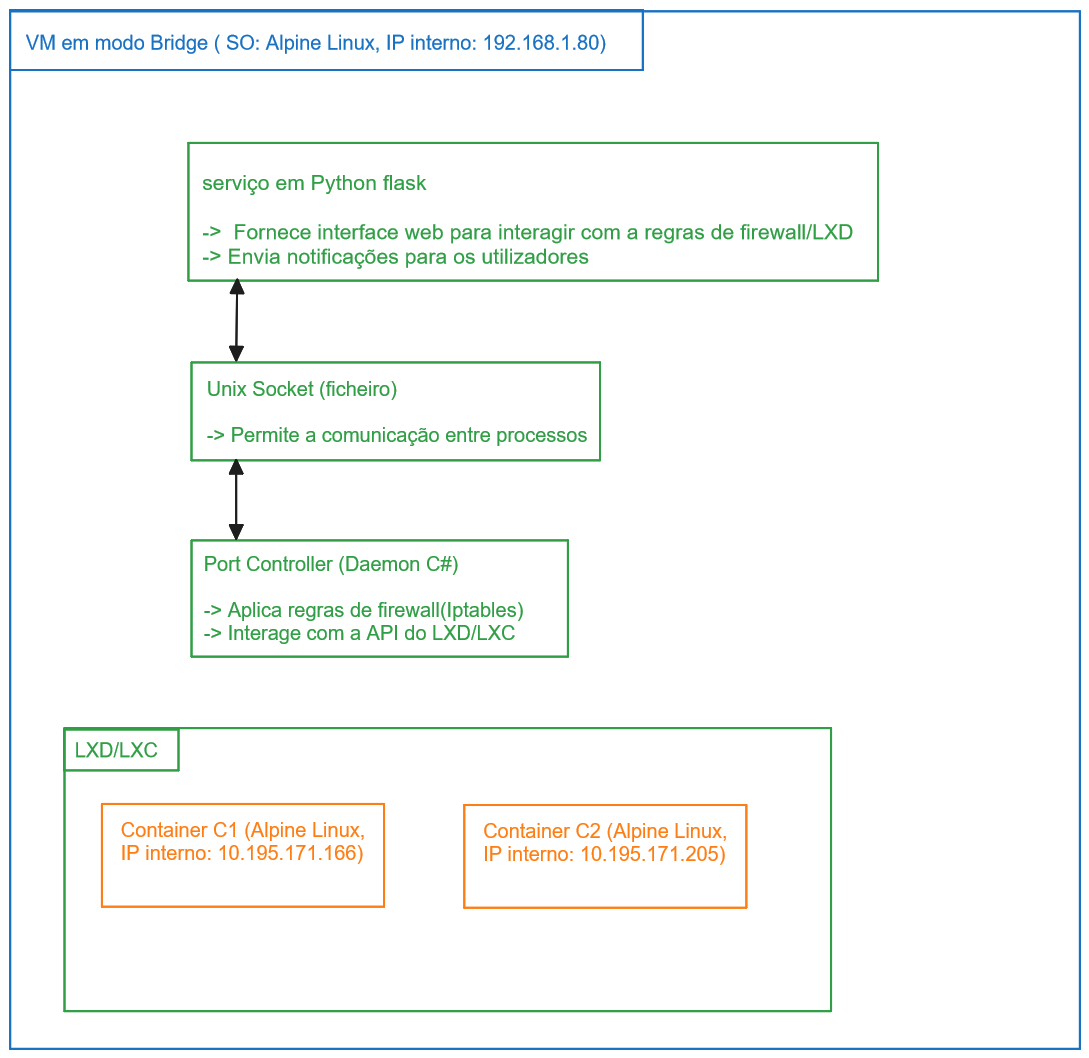
\includegraphics[width=14cm]{figs/estrutura2.png}
\caption{Abiente do projeto}
\label{fig:bookstack}
\end{center}
\end{figure}



\section{Ambiente de testes do projeto}

Esta secção do relatório irá abordar os passos efetuados na configuração do sistema 
usado como ambiente de testes do projeto e respetivas aplicações/pacotes instalados.

Sendo os seguintes:
\begin{enumerate}
    \item Configuração do Alpine Linux;
    \item Configuração do LXD/LXC;
    \item Instalação do .NET Core;
    \item Instalação de outros pacotes;
\end{enumerate}


\subsection{Configuração do Alpine Linux}

De modo a obter, os melhores resultados possiveis durate os estes e experiencias
ao longo deste projeto é de extrema importância que o sistema operativo de testes
seja o mesmo da plataforma Forge. Sendo assim foi intalada numa máquina virtual
VMware com o alpine linux 3.19.

Especificações atribuidas à maquina virtual:

\begin{itemize}
    \item 6 GB de RAM;
    \item 3 nucleos de para o CPU;
    \item Placa de rede no modo Bridge;
    \item 40 GB de armazenamento;
\end{itemize}

De seguida foi feita a configuração inicial do sistema com os seguintes coamandos:


\begin{enumerate}
    \item \texttt{localhost login: root 
    \item setup-alpine
    \item Select keyboard layout: pt-pt
    \item Enter a system hostname : alpine
    \item Which one do you want to initialize? [eth0]
    \item Ip address for eth0? [dhcp]
    \item Do you want to do any manual network configuration? (y/n) [n] n
    \item (Changing password for root) New password: ******
    \item which timezone are you in [UTC]
    \item HTTP/FTP proxy URL? [none]
    \item Enter mirror number (1-72) or URL to add (or r/f/e/done) [1]
    \item Setup user? (enter a lower-case loginname, or 'no') [no] delta
    \item Password: ******}
    \item Enter ssh key or URL for titus (or 'none') [none]
    \item Which ssh server ('openssh', 'dropbear', or 'none') [openssh]
    \item Which disk(s) would you like to use? [none] sda 
    \item how you would like to use it? ('sys', 'data', 'crypt', 'lvm' or '?'for help) [?] sys 
    \item Erase the above disk(s) and continue? (y/n) [n] y 
    \item Instalation Complete. Please reboot.
\end{enumerate}


\textbf{Nota:} As opcções \textit{default} são sugeridas dentro de "[]" caso se pretenda
usar essa opção é apenas necessário carregar na tecla "\textit{ENTER}". \\


Para terminar a configuração foi executado o comando: 

%\texttt{apk add --upgrade apk-tools \&\& apk upgrade --available} \\

\begin{tcolorbox}[colback=blue!5!white,colframe=blue!75!black]
    \verb |doas apk add --upgrade apk-tools \&\& apk upgrade --available |
\end{tcolorbox}

Foi também ativado o repositório da comunidae para ter um maior
numero de pacotes para instalar. Para isto é necessário descomentar a linha no
ficheiro "\textit{repositories}" com a localização "/etc/apk/repositories" com o
URL deste repositório, removendo o "\#" no inicio da linha.

No final o conteúdo do ficheiro deverá ser este:

\begin{lstlisting}[language=Bash, caption={Ficheiro repositories}]
http://dl-cdn.alpinelinux.org/alpine/v3.19/main
http://dl-cdn.alpinelinux.org/alpine/v3.19/community
\end{lstlisting}

\subsection{Configuração do LXD/LXC}

No que diz respeito ao LXD/LXC foram instalados os pacotes lxd e lxd-client.


Foi ativado o serviço do lxd como default com o comando \texttt{rc-update add lxd default}
e em seguida ativado com o \texttt{rc-service lxd start}.

Depois foi feita a configuração iniciul com o comando texttt{lxd init} com a seguintes opções:

\begin{enumerate}
    \item \texttt{Would you like to use LXD clustering? (yes/no) [default=no]: no
    \item Do you want to configure a new storage pool? (yes/no) [default=yes]: yes
    \item Name of the new storage pool [default=default]: default
    \item Name of the storage backend to use (btrfs, dir, lvm, zfs) [default=zfs]: dir
    \item Would you like to connect to a MAAS server? (yes/no) [default=no]: no;
    \item Would you like to create a new local network bridge? (yes/no) [default=yes]: yes
    \item What should the new bridge be called? [default=lxdbr0]: lxdbr0
    \item What IPv4 address should be used? (CIDR subnet notation, “auto” or “none”) [default=auto]: auto
    \item What IPv6 address should be used? (CIDR subnet notation, “auto” or “none”) [default=auto]: auto
    \item Would you like LXD to be available over the network? (yes/no) [default=no]: no
    \item Would you like stale cached images to be updated automatically? (yes/no) [default=yes] yes
    \item Would you like a YAML "lxd init" preseed to be printed? (yes/no) [default=no]: no}
\end{enumerate}

De seguida foi editada a configuração \textit{default} com o 
comando "\texttt{lxc profile edit default}" nela deverá ser garantida o
seguinte:

\begin{lstlisting}[language=csh, caption={edição do perfil padrão}]
  eth0:
    name: eth0
    nictype: bridged
    parent: lxdbr0
    type:nic

\end{lstlisting}

\textbf{Nota:} eth0 é a interface do sistema \textit{host} e lxdbr0 é a interface
de rede criada automaticamente pelo LXD.

Com esta configuração os \textit{containers} irão funcionar em modo NAT.


Após isto foram criados dois containers Alpine linux com o seguinte 
comando: % "\texttt{lxc launch images:alpine/3.19 <nome do container>}"

\begin{tcolorbox}[colback=blue!5!white,colframe=blue!75!black]
    \verb |doas lxc launch images:alpine/3.19 <nome do container> |
\end{tcolorbox}

Podendo assim serem listados com o comando:

\begin{tcolorbox}[colback=blue!5!white,colframe=blue!75!black]
    \verb |doas lxc list |
\end{tcolorbox}


A seguinte imagem mostra o output do comando acima referido.

\begin{figure}[H]
\begin{center}
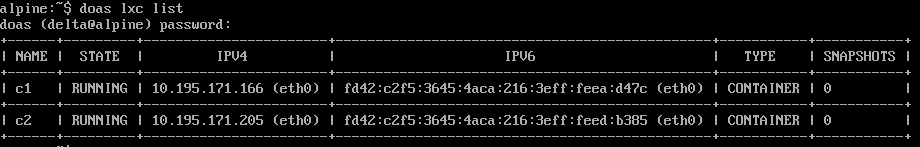
\includegraphics[width=14cm]{figs/lista de containers.png}
\caption{Containers criados.}
\label{fig:bookstack}
\end{center}
\end{figure}



\subsection{Instalação do .NET Core}


Para depois poder executar a aplicação que irá controlar as portas dos containers,
aplicação esta desenvolvida em C\# .NET Core é necessário instalar os pacotes necessários
para o funcionamento da mesma, mais concretamente o sdk e o \textit{runtime}.

Os pacotes necessŕios foram instalados usando os seguintes comandos:
\begin{itemize}
    \item \texttt{doas apk add dotnet7-sdk};
    \item \texttt{doas apk add dotnet7-runtime};
\end{itemize}




\subsection{Instalação de outros pacotes}

Para além do .NET Core, para garantir o funcionamento das aplicações desenvolvidas neste projeto é necessário
instalar ainda os seguintes pagotes:
\begin{itemize}
    \item Python - \texttt{doas apk add python3};
    \item Pip - \texttt{doas apk add python3-pip}
    \item Bash - \texttt{doas apk add bash};
\end{itemize}


Para uma maior facilidade de uso do sistema durante o seu uso foi também instalado
o "tmux" que permite criar "janelas" e trocar rapidamente entre as mesma, funcionalidade
essa que aumenta a produtividade num ambiente de apenas terminal.
Para asua instala ção foi usado o comando:
\begin{itemize}
    \item \texttt{doas apk add tmux};
\end{itemize}







%==========================================================================


\section{Testes de Firewall e conexões realizados}

Uma vez os \textit estarem configurados em modo NAT seria necessário criar regras 
de redirecionamento de portas ou endereços IP de modo a os \textit{containers} serem acedidos
por outros dispositivos na rede local.


De modo a realizar testes de conexão foram instalados dentro dos containers
o netcat e o python.

\textbf{Nota:} eth0 é a placa de rede do sistema host e tem o ip local de 192.168.1.80.


Durante os testes realizados, concluiu-se que existem três medodos de criar conectividade:

\subsection{Método 1: Criar regras no lxc network e defenir portas de redirecionamento}

\textbf{Nota:} Neste metodo será usado como exemplo o \textit{container} "c2" que
dentro da máquina virtual host tem o IP 10.195.171.166.

\textbf{Nota nº2:} A máquina virtual \textit{Host} tem o endereço IP 192.168.1.80.

Este metodo usa o comando "\texttt{lxc network forward create lxdbr0 192.168.1.80}"
para criar a regra e "\texttt{lxc network forward port add lxdbr0 192.168.1.80 tcp 7000 10.195.171.205 8000}"
para adicionar as portas a serem reencaminhadas, neste exemplo o trafego vindo da
rede local que tenta aceder ao endereço IP 192.168.1.80 (\textit{host}) pela porta 7000 será redirecionado
para a porta 8000 do IP 10.195.171.205 que pertence ao container "c2".

Nesta experiência o container está a executar um servidor http na porta 8000
com o comando "\texttt{python3 -m http.server}".


\textbf{Nota:} Porta 8000 é a padrão quando não é especificada outra no final do comando.


Foi possivel aceder ao servidor HTTP pelo browser num computador da rede local.

\begin{figure}[H]
\begin{center}
\includegraphics[width=12cm]{figs/teste de conexão via browser.png}
\caption{Teste de conexão via browser.}
\label{fig:bookstack}
\end{center}
\end{figure}


Foram também usados alguns comandos do netcat como o seguinte: % "\texttt{nc -w1 -vz 192.168.1.80 7000}".

\begin{tcolorbox}[colback=blue!5!white,colframe=blue!75!black]
    \verb | nc -w1 -vz 192.168.1.80 7000 |
\end{tcolorbox} 


\begin{figure}[ht]
\begin{center}
\includegraphics[width=12cm]{figs/teste de conexão1.png}
\caption{Teste de conexão com o netcat.}
\label{fig:bookstack}
\end{center}
\end{figure}

Foram usados também usados os comandos "\texttt{nc 192.168.1.80 7000} e \texttt{nc -l 8000}"
de modo a criar uma ligação TCP. Foi também testado a ligação reversa
onde o \textit{container} se tenta ligar ao computador da rede, invertendo os comandos
"\texttt{nc 192.168.1.68 3000}" e "\texttt{nc -l 3000}", ambos os testes foram bem
sucedidos.







\subsection{Método 2: Usar um IP para redirecionar o tráfego para o container}

Neste método é atribuido um endereço ip da rede local, que esteja disponivel, à
interface de rede do sistema host, eth0, usado o comando
"\texttt{ip address add 192.168.1.120/24 dev eth0}", para este exemplo foi escolhido o IP
"192.168.1.120".

De seguida, é necessário criar a regra de redirecionamento do tráfego
com o IP de destino "192.168.1.120" para o IP de um \textit{container}, que neste esxemplo será o
IP "10.195.171.166" que pertence ao \textit{container} "c1", para isto foi usado o
comando "\texttt{lxc network forward create lxdbr0 192.168.1.120 target\_address=10.195.171.166}"
que automaticamente cria uma regra na tabela NAT do iptables para garantir o correto
funcionamento do redirecionamento.

Com esta configuração se o \textit{container} "c1" que possui o IP "10.195.171.166" estiver a executar um servidor 
http na porta 8000, o mesmo serviço estará disponivel para dispositivos da rede local
através do IP 192.168.1.120 na porta 8000.

\textbf{Nota:} Os testes de conexão usados no método 1 foram igualmente bem sucedidos.


Após usar o comando "\texttt{lxc network create <network name> <listen address>}", é ainda possivel pecificar portas com o seguinte comando:

\begin{tcolorbox}[colback=blue!5!white,colframe=blue!75!black]
    lxc network forward port add $<$network\_name$>$ $<$listen\_address$>$ $<$protocol$>$ $<$listen\_ports$>$ $<$target\_address$>$ $[<$target\_ports$>]$
\end{tcolorbox}

O seguinte exemplo mostra a associação do IP do \textit{container} da porta 22 com a porta 22 do IP externo atribuído (192.168.1.120).

\begin{tcolorbox}[colback=blue!5!white,colframe=blue!75!black]
    lxc network forward port add lxdbr0 192.168.1.120 tcp 22 10.195.171.166 22
\end{tcolorbox}

\subsection{Método 3: Usar o Iptables para criar portas de redirecionamento}

O método 3 é o mesmo que o médotos anteriores mas só que configurado usando apenas regras
do Iptables, ou seja, é criaca uma regra na tablea NAT que redireciona o tráfego
de uma porta do sistema host para um IP e porta de um \textit{container}.

É possivel criar esta configuração com o comando:



%\begin{lstlisting}[language=Bash, caption={Exemplo de regra de redirecionamento}]
%    doas iptables -t nat -I PREROUTING -p tcp --dport 5000 -j DNAT --to-destination 10.195.171.205:8000
%\end{lstlisting}

\begin{tcolorbox}[colback=blue!5!white,colframe=blue!75!black]
    doas iptables -t nat -I PREROUTING -p tcp --dport 5000 -j DNAT --to-destination 10.195.171.205:8000
\end{tcolorbox}

Neste exemplo similar ao exemplo do método 1, se o \textit{container} "c2" com o 
endereço IP "10.195.171.205", estiver a executar um servidor HTTP na porta
8000, os dispositivos na rede local poderão aceder a este serviço acedendo à porta 
5000 do IP do sistema host(192.168.1.80).


Da mesma forma que o método 2 è possivel associar também um IP externo com o seguinte comando de exemplo
onde é feita a associação da porta 22 juntamente com o ip externo atribuído:

Importante referir, que antes deste de criar a regra no iptables é necessário usar o
comando ”\texttt{ip address add 192.168.1.120/24 dev eth0}”, para adicionar o endereço IP
à placa de rede do sistema.

\begin{tcolorbox}[colback=blue!5!white,colframe=blue!75!black]
    doas iptables -t nat -I PREROUTING -p tcp --dport 22 -d 192.168.1.120 -j DNAT --to-destination 10.195.171.166:22
\end{tcolorbox}



\textbf{Nota:} Os testes de conexão usados no método 1/2 foram igualmente bem sucedidos.




% =============================================================================
% =============================================================================



\section{Testes da API do LXD}


Após os testes referidos na secção anterior, terem sido concluídos, foi necessário
reproduzir os mesmos resultados, mas com a API do LXD.

A vantagem principal em usar este método está na performance da interação do "Port Controller" com
o LXC, que no momento de criar uma regra, será criado menos um processo, do que 
usar o "Port Controller" para executar um comando do LXC/LXD na \textit{shell} do sistema.

Portanto, após consultar a \href{https://documentation.ubuntu.com/lxd/en/latest/api/#/}{documentação oficial da API do LXD},
nomeadamente, a secção "network-forwards" foram realizados com sucesso, auxilio do comando curl, os seguintes testes:


Importante referir que para um melhor funciuonamento da API e de modo a evitar erros,
é recomendado os endereços IP, que se prentendam atribuir a um \textit{container} 
sejam previamente adicionados e associados ao "LXC forward" com um dos seguintes comandos:

\begin{tcolorbox}[colback=blue!5!white,colframe=blue!75!black]
    lxc network forward create $<$network\_name$>$ $<$listen\_address$>$
\end{tcolorbox}

\begin{tcolorbox}[colback=blue!5!white,colframe=blue!75!black]
    lxc network forward create lxdbr0 192.168.1.120
\end{tcolorbox}


ou com o curl e com o IP "192.168.1.120" a servir de IP externo:


\begin{lstlisting}[language=Bash, caption={Exemplo para registar um IP para redirecionar trafego (API do LXD)}]
    curl --unix-socket /var/lib/lxd/unix.socket -X POST -d '{"config":{},"description":"","listen_address":"192.168.1.120","ports":[]}'  lxd/1.0/networks/lxdbr0/forwards
\end{lstlisting}


Após isso, exclusicamente através da API do LXD é necessário associar o IP externo previamente
adicionado com o endereço IP do \textit{container} e respetivas portas.

É possivel realizar esta operação com uma solicitação "PUT" para a API do LXD

\begin{lstlisting}[language=Bash, caption={Exemplo de associação de IPs e portas usando a API do LXD}]
    curl --unix-socket /var/lib/lxd/unix.socket -X PUT -d '{"config":{},"description":"10.195.171.166","listen_address":"192.168.1.120","ports":[{"description":"","listen_port":"7000","protocol":"tcp","target_address":"","target_port":"8000"}]}'  lxd/1.0/networks/lxdbr0/forwards/192.168.120
\end{lstlisting}


No exemplo acima é criada a associação entre a potra 8000 do IP "10.195.171.166" que pertence a 
um \textit{container} e a porta 7000 do IP externo "192.168..1.120".

Uma fez realizado com sucesso este teste será apenas necessário implementar esta 
mesma solicitação no "Port Controller". \\






\textbf{Nota:} Caso se pretenda criar conexão exclusivamente através de IPs sem especificar portas é 
possivel, no momento de adição do IP externo ao "LXD forward" usar a seguinte comando:

\begin{lstlisting}[language=Bash, caption={Exemplo para registar um IP e associá-lo a um cinatiner (API do LXD)}]
    curl --unix-socket /var/lib/lxd/unix.socket -X POST -d '{"config":{"target_address":"10.195.171.166"},"description":"","listen_address":"192.168.1.120","ports":[]}'  lxd/1.0/networks/lxdbr0/forwards
\end{lstlisting}

Esta solicitação efetuada com o curl tem o mesmo resultado do comando:

\begin{tcolorbox}[colback=blue!5!white,colframe=blue!75!black]
   lxc network forward create lxdbr0 192.168.1.120 target\_address=10.195.171.166
\end{tcolorbox}








% =============================================================================
% =============================================================================


\section{Criação da REST API}

Para interagir com o daemon C\# (Port Controller) responsável por interagir com regras do iptables
e configurações do LXC/LXD, foi criada uma API em Python com a biblioteca Flask como
método alternativo à interface \textit{Web}.

O principal motivo da criação desta API é a facilitação nos momentos de teste dos programas
desenvolvidos, uma vez que pode ser testada no terminal com o comando Curl. Contudo, nada 
impede o administrador do sistema de usar este método de interação com o "Port Controler"
como forma principal, uma vez que funciona de formna independente da interface Web.

Sendo assim, neste componente do projeto desenvolvida em Python à três partes essênciais:

\begin{enumerate}
    \item API - que permite ao utilizador (administrador do sistema) interagir com o "Port Controller" daemon em C\#
    através do terminal fazendo solicitações HTTP com o comando Curl;
    \item Interface Web - que permite ao utilizador (administrador do sistema) interagir com o "Port Controller"
    através de uma interface gráfica que pode ser acedida através do \textit{browser};
    \item O ficheiro (unixSocketConn.py) que comunica com a unix socket (localizada em /tmp/socket\_proj) que por sua vez, comunica com o "Port Controller". 
\end{enumerate}

Nesta secção o foco será a explicação do funcionamento da API, porém, para esclarecer
melhor o funcionamentodos ficheiros referidos a seguinte imagem
mostra o fluxo de comunicação entre os ficheiros/programas do projeto.

\begin{figure}[H]
\begin{center}
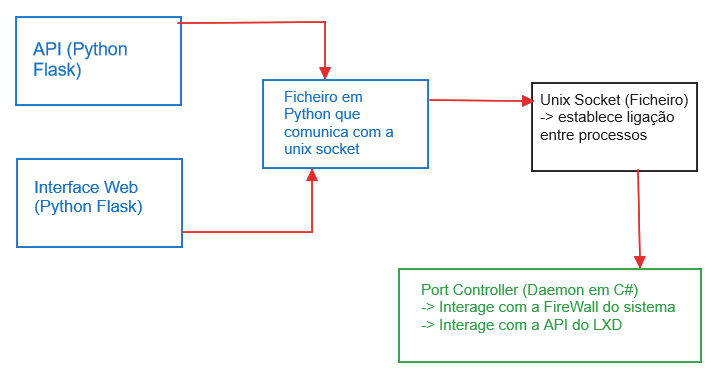
\includegraphics[width=14cm]{figs/fluxo de comunicação.png}
\caption{Fluxo de comunicação do projeto}
\label{fig:bookstack}
\end{center}
\end{figure}



\subsection{Pré-requesitos}

Uma vez que esta componte de API de projeto é feita usando a linguagem Python é necessário
usar as seguintes bibliotecas:

\begin{itemize}
    \item Flask - biblioteca responsável pela criação da API;
    \item re - biblioteca usada para expressões regulares;
    \item json - biblioteca para manipulação de contúdo em fm formato JSON;
\end{itemize}
    
Das bibliotecas mencionadas apenas o "Flask" é externa, sendo necessário instalar a mesma
com o seguinte comando:

\begin{tcolorbox}[colback=blue!5!white,colframe=blue!75!black]
    \verb | doas apk add py-flask |
\end{tcolorbox}

\textbf{Nota:} O Alpine linux não permite instalar bibliotecas/pacotes usando o "pip" (gestor de pacotes
do python) de forma direta.

Após intalado é necessário garantir as seguintes linhas no ficheiro "main" da API.

\begin{lstlisting}[language=csh, caption={Importações necessárias}]
from flask import Flask, request, jsonify
import re
import json
from unixSocketConn import *
\end{lstlisting}

A linha 4 é faz importação das funções defenidas do ficheiro "unixSocketConn.py", ficheiro esse, 
responsável for enviar dados para o ficheiro da unxix socket.




\subsection{Estrutura da API}

A API está dividida em três partes/caminhos URL:

\begin{enumerate}
    \item  \slash host\_fw - onde as solicitações feitas para este URL serão relacionadas à interação
    com a Firewall do sistema, mais concretamnte a tabela Filter do Iptables\slash Nftables;
    \item  \slash host\_nat - neste caminho as solicitações são relacionadas à interação com
    com a Firewall do sistema mas direcionadas à tabela NAT ou regras do LXD Forward;
    \item  \slash cont\_port (caminho secundário/opcional) - Neste caminho as solicitações, têm o objetivo de interagir com regras de firewall
    (Iptables ou nftables) dentro de \textit{containers} alojados dendoro do sistema \textit{host}. 
\end{enumerate}


\title*{\textbf{Exemplo de código}}

No seguinte excerto de código mostra um a implementação de um caminho da API (\slash host\_nat)

\begin{lstlisting}[language=Bash, caption={Definição de um caminho}]
@app.route("/host_fw", methods=["POST"]) # executar no host
def host_fw():
    
    try:

        data = request.get_json()
        
        action = data['Action']
        firewall = data['Fw']
        protocol = data['Protocol']
        porta = data['Port']

    except:
        print("Erro ao receber dados!")
        return "Error ao receber os dados", 500
    else:

        hostfw(action, firewall, protocol, porta)
        
        return jsonify(data, "Solicitacao bem sucedida!"), 201  
\end{lstlisting}

Neste excerto de código está a função responsável por receber a solicitação \textit{POST}.
Dentro da secção do "try" os valores enviados em JSON pela solicitação serão guardados em
variáveis para depois serem passados para a função "hostfw" função essa que percente ao ficheiro
"unixSocketConn.py". As funções presentes neste ficheiro após receberem os valores vindos 
da solicitação enviam os dados formatados em JSON para o ficheiro da unix socket (/tmp/socket\_proj) que por sua vez,
chegará ao "Port controller".



\subsection{Definição dos parâmetros}

Para fazer uma solicitação para um destes caminho foram defenidos parâmetros\slash argumentos
que podem ser enviados, os mesmos podem visualizados na seguinte tabela:

\begin{table}[H]
\centering
\begin{tabular}{|c|c|}
\hline
\rowcolor{yellow!50}\textbf{Parâmetros} & \textbf{Opções}\\
\hline
Container & $<$Container name$>$\\
\hline
Type & lxc, incus \\
\hline
Action & ClosePort, OpenPort, AddNat, RemoveNat, ResetNat, ExecCmd \\
\hline
Fw & ipt, nft, lxcforward, lxdapi \\
\hline
Port & $<$numero entre 1-65535$>$ \\
\hline
protocol & tcp, udp \\
\hline
Container\_internal\_ip & $<IP>$ \\
\hline
Container\_internal\_port & $<$numero entre 1-65535$>$ \\
\hline
Rule & $<$Regra costumizada e opcional para usar na Firewall(Iptables ou Nftables)$>$ \\
\hline
\end{tabular}
\caption{Lista de parâmetros possiveis de usar.}
\label{arglist}
\end{table}

\textbf{Nota:} Os parâmetros não são todos obrigatórios, alguns dependem do URl para o qual
se pretende fazer solicitação.


\subsection{Formato da solicitação}

Para fazer uma solicitação para um URL da API será usado o comando curl como exemplo para
cada um dos caminhos criados.

As solicitações devem ser feitas deve ser do tipo POST de modo a enviar dados com os parãmetros
corretos para aquele aquele caminho e em formato JSON.

Com comando "curl" é especificado o tipo de solicitação com a "flag" \texttt{-X <tipo de solicitação>},
o cabeçalho com a "flag" \texttt{-H "<Conteúdo do cabeçalho>"}, de seguida com a "flag" -d os parâmetros
em formato JSON dentro de aspas simples e por fim, o URL completo para o qual se prentende enviar a
solicitação.



\title*{Exemplo para \slash \textbf{host\_fw}}

\begin{lstlisting}[language=Bash, caption={Exemplo de solicitação para a firewal do sistema host}]
    curl -X POST -H "Content-Type:application/json" -d '{"Action":"OpenPort","Fw":"ipt","Protocol":"tcp","Port":"22"}' http://localhost:5000/host_fw
\end{lstlisting}



Como se pode observar neste exemplo para o caminho "host\_fw" os parâmetros passados devem ser:

\begin{enumerate}
    \item Action;
    \item Fw;
    \item protocol;
    \item Port;
    \item Rule (Opcional);
\end{enumerate}

Opcionalmente é possivel usar o parâmetro "Rule" e especificar uma regra para o Iptables\slash Nnftables
para tal o parâmetro "\textit{Action}" deve ser "ExecCmd", o parâmetro "Fw" deve ser referido normalmente com "ipt" ou "nft" e os restantes devem ser mencionados mas vazios, como no seguinte exemplo:

\begin{lstlisting}[language=Bash, caption={Exemplo de solicitação para a firewal do sistema host com uma regra personalizada}]
    curl -X POST -H "Content-Type:application/json" -d '{"Action":"ExecCmd","Fw":"ipt","Protocol":"","Port":"", "Rule":"INPUT -s 192.168.1.140 -j DROP"}' http://localhost:5000/host_fw
\end{lstlisting}



\title*{\textbf{host\_nat}}

\begin{lstlisting}[language=Bash, caption={Exemplo de solicitação para a firewal do sistema host para associar um IP externo a umIp de container de modo a criar conectividade}]
    curl -X POST -H "Content-Type:application/json" -d '{"Action":"AddNat","Fw":"ipt","Protocol":"tcp","Port":"22","External_ip":"192.168.1.120","Container_internal_ip":"10.195.171.205","Container_internal_port":"80" }' http://localhost:5000/host_nat
\end{lstlisting}

Neste exemplo pretende-se criar conectividade criando uma regra na tabela NAT do iptables de modo a associar
um IP interno de um \textit{container} com um IP externo escolhido pelo administrador do sistema.

É possivel executar o comando comando de igual forma trocando apenas o parâmetro "Fw" para "lxdforward" 
ou "lxdapi" de modo a criar a mesma associação mas através do LXD, tanto um como outro criará uma regra
semelhante ao Iptables de forma automática.

A vantagem principal está em usar a opção "lxdapi", que como nome indica irá usar a API do LXD para
criar a regra, que em comparação com as outras opções garante performance extra uma vez que não é necessária
a criação de um novo processo para criar uma regra. De qualquer forma este tópico será abordado e explicado mais detalhadamente 
na secção de explicação do "Port Controller". \\


\title*{\textbf{cont\_port}}

\begin{lstlisting}[language=Bash, caption={Exemplo de solicitação para a firewal do sistema host para associar um IP externo a umIp de container de modo a criar conectividade}]
    curl -X POST -H "Content-Type: application/json" -d '{"Container":"c1","Type":"lxc","Action":"OpenPort","Fw":"ipt", "Protocol":"tcp","Port":"22"}' http://localhost:5000/cont_port
\end{lstlisting}

Com uma estrutura similar à solicitação feita para o "host\_fw", as solicitações para o caminho "cont\_port"
devem apenas incluir os parâmetros "Container" e "Type".
\begin{enumerate}
    \item Container;
    \item Type;
    \item Action;
    \item Fw;
    \item protocol;
    \item Port;
    \item Rule (Opcional);
\end{enumerate}




\subsection{ligação à unix socket}

O seguinte excerto de código mostra como funciona uma função no ficheiro "unixSocketConn.py" responsável
para se ligar à unix socket, localizada em "/tmp/socket\_proj" (localização da unix socket
é opcional) e assim enviar os dados atrvés da mesma para o "Port Controller".

\begin{lstlisting}[language=Bash, caption={Definição de um caminho}]
def hostfw(action, firewall, protocol, porta):

socket_path = socketPath()

try:
    # Criar uma Unix socket
    client_socket = socket.socket(socket.AF_UNIX, socket.SOCK_STREAM)

    # Conectar a Unix socket
    client_socket.connect(socket_path)

    # Enviar uma mensagem para o servidor
    
    json_data = {
        "Type": "host",
        "Action": action,
        "Fw": firewall,
        "Protocol": protocol,
        "Port": porta
    }
    
    client_socket.send(json.dumps(json_data).encode())


    time.sleep(1.5)
    # Receber a resposta 
    response_json = client_socket.recv(1024).decode()
    response = json.loads(response_json)

    # mostrar a resposta
    print("Status:", response["Status"])
    print("Mensagem:", response["Mensagem"])

    # Fechar o socket
    client_socket.close()

except Exception as e:
    print("Ocorreu um erro:", e)  
\end{lstlisting}


É possivel observar la linha 7 a definição do tipo se socket e o tipo de transferênia,
na linha 14 é defenida a estrura em JSON que será envida, nela o paraaâmetro "Type" é 
defenida como "host" de modo a informar o "Port Controller" que é o alvo do comando/regra a ser
executado é o próprio sistema \textit{host}.

De seguida, na linha 22 a estrutura json é formatada e envida para a unix socket.

O código seguinte é responsável por receber a resposta do "Port Controller", por fim, a conexão
é com a unix socket é fechada na linha 35. 










% =============================================================================

\section{Port Controller}

\subsection{Escolha da tecnologia}

Uma vez que a plataforma forge funciona no sistema \textit{Alpine Linux} seria
necessário escolher ferramentas suportadas por esta distribuição.

No caso desta parte do projeto, foi escolhida a linguagem C\# com o 
\textit{framework} .NET Core versão 7.0.



\subsection{Funcionalidades}

"Em sistemas operativos de computador multitarefa, um daemon é um programa de 
computador executado como um processo em segundo plano, em vez de estar sob o 
controle direto de um utilizador interativo. Tradicionalmente, os nomes dos processos
de um daemon terminam com a letra d, para esclarecer que o processo é de fato um 
daemon e para diferenciar entre um daemon e um programa de computador normal." \cite{daemon}

Este componente do projeto, denominado de "Port Controller", tem como objetivo,
funcionar constantemente em segundo plano, para controlar as conexões ao
sistema\textit{host} e dos \textit{containers} nele alojados.

O \textit{"Port Controller"} tem como principal função estar à escuta de pedidos
do administrador e executar estes pedidos na \textit{Firewall} do sistema
\textit{host} (Iptables) ou a API do LXD de modo a gerir conexões relacionadas 
com os \textit{containers} ativos ou ao próprio sistema \textit{host}.
Os pedidos são recebidos na componente da \textit{unix socket} em formato
\textit{JSON}.


Opcionalmente, o \textit{"Port Controller"} é também capaz de interagir com \textit{containers}
do tipo LXC e executar comandos dentro destes para interagir com a
\textit{Firewall} Iptables ou Nftables.

\subsection{Estrutura do código}

O código do "Port Controller" é constituido pelos seguintes ficheiros:

\begin{itemize}
    \item Program.cs;
    \item SocketData.cs;
    \item Firewall.cs
    \item Container.cs
    \item Lxc.cs

\end{itemize}


\subsection{Funcionamento do código}

\title*{\textbf{Program.cs}}

No Ficheiro Program, na função \textit{main} está defenido o caminho do ficheiro 
da unix socket que permite a comunição entre o \textit{"Port Controller"} e 
a interface \textit{Web} ou API.


\begin{lstlisting}[language=csh, caption={verificação da existência da unix socket}]
// Caminho do ficheiro do socket
string socketPath = "/tmp/socket_proj";

if (File.Exists(socketPath))
{
    Console.WriteLine("O ficheiro do socket ja existe. A criar um novo...");
    File.Delete(socketPath);
}

\end{lstlisting}

Neste excerto de código é feita uma verificação, se o ficheiro já existe e se sim, este será apagado,
para depois ser criado um novo.\\



O seguinte excerto de código mostra a criação de uma nova instância de uma \textit{Socket}
(linha 2), a ligação ao ficheiro da unix socket é feito na linha 7.

\begin{lstlisting}[language=csh, caption={ligação do Port Controller à unix socket}]
// Criar a unix socket
Socket serverSocket = new Socket(AddressFamily.Unix, SocketType.Stream, ProtocolType.Unspecified);

try
{
    // ligar o socket a unix socket
    serverSocket.Bind(new UnixDomainSocketEndPoint(socketPath));

    // Definir o tamanho maximo da fila de conexoes pendentes
    serverSocket.Listen(5);

    Console.WriteLine("A espera de pedidos...");

    // Loop para aceitar conexaes
    while (true)
    {
        // Aceitar a conexao do cliente
        Socket clientSocket = serverSocket.Accept();

        SocketData data = new SocketData();

        Thread thread = new Thread(() => data.ReceberJson(clientSocket));
        thread.Start();
    }

}
catch (Exception ex)
{
    Console.WriteLine($"Ocorreu um erro: {ex.Message}");
}
finally
{
    // Fechar o socket
    serverSocket.Close();
}
\end{lstlisting}

Na linha 15 está um ciclo que aceita conexões e os dados recevbidos da conexão
são enviados para um função "ReceberJson" (que pertence à classe "SocketData") 
numa nova \textit{thread}, conseguindo assim, executar múltiplos 
pedidos em simultâneo. \\


\title*{\textbf{SocketData.cs}}


Nesta classe "Socketdata" está presente a função "ReceberJson", responsável por ler 
os dados recebidos da API ou da interface \textit{web} através da unix socket.

\begin{lstlisting}[language=csh, caption={Leitura dos dados recebidos}]
// Ler os dados recebidos do cliente(socket)
byte[] buffer = new byte[1024];
int bytesRead = clientSocket.Receive(buffer);
string jsonData = Encoding.UTF8.GetString(buffer, 0, bytesRead);
dynamic receivedData = JsonConvert.DeserializeObject(jsonData);

// Imprime os dados recebidos
Console.WriteLine("Dados recebidos do client:");
Console.WriteLine($"Nome: {receivedData.Container}");
Console.WriteLine($"Type: {receivedData.Type}");
Console.WriteLine($"Action: {receivedData.Action}");
Console.WriteLine($"Firewall: {receivedData.Fw}");
Console.WriteLine($"Protocol: {receivedData.Protocol}");
Console.WriteLine($"Port: {receivedData.Port}");
Console.WriteLine($"External_ip: {receivedData.External_ip}");
Console.WriteLine($"Container_internal_ip: {receivedData.Container_internal_ip}");
Console.WriteLine($"Container_internal_port: {receivedData.Container_internal_port}");
Console.WriteLine($"Rule: {receivedData.Rule}");

// conversao das variaveis para string
string scont_name = receivedData.Container;
string stype = receivedData.Type;
string saction = receivedData.Action;
string sfw = receivedData.Fw;
string sprotocol = receivedData.Protocol;
string sport = receivedData.Port;
string sexternal_ip = receivedData.External_ip;
string scont_internal_ip = receivedData.Container_internal_ip;
string scont_internal_port = receivedData.Container_internal_port;
string srule = receivedData.Rule;
\end{lstlisting}  


De seguida, conforme os dados recebidos é determinado qual ação o programa deve executar,
passado pela seguinte sequência de "ifs"

\begin{lstlisting}[language=csh, caption={Opções possiveis em Firewall.cs}]
if (receivedData.Type == "host" && receivedData.Action == "ClosePort" || receivedData.Type == "host" && receivedData.Action == "OpenPort" || receivedData.Type == "host" && receivedData.Action == "ExecCmd")
{
    clientSocket.Close();
    
    Firewall fwh = new Firewall();

    fwh.AddRule(saction, sfw, sprotocol, sport, srule);
}
if (receivedData.Type == "host" && receivedData.Action == "AddNat" || receivedData.Type == "host" && receivedData.Action == "RemoveNat" || receivedData.Type == "host" && receivedData.Action == "ResetNat")
{  
    clientSocket.Close();

    Firewall fwn = new Firewall();

    fwn.AddRuleNat(saction, sfw, sprotocol, sport, sexternal_ip, scont_internal_ip, scont_internal_port, srule);

}
if (receivedData.Type == "lxc" || receivedData.Type == "incus")
{
    clientSocket.Close();

    switch (stype)
    {
        case "lxc":
            Console.WriteLine("Opcao 1 selecionada.");

            Lxc lxc = new Lxc();

            lxc.AddRule(scont_name, saction, sfw, sprotocol, sport, srule);

            break;
        case "incus":
            Console.WriteLine("Opcao 2 selecionada.");

            Incus incus = new Incus();

            incus.AddRule(scont_name, saction, sfw, sprotocol, sport, srule);

            break;
        default:
            Console.WriteLine("Opcao invalida. (execRegraContainer)");
            break;
    }
}
clientSocket.Close();

\end{lstlisting}  

Neste excerto código, são verificados os dados recebidos, caso estes se destinem a 
instruções para a \textit{firewall} do sistema o primeiro "if" será executado, se forem dados relacionados
à adição de regras NAT será executado o segundo "if" e por fim se o objetivo for executar comandos de
\textit{firewall} dentro de um \textit{container} será o terceiro "if" executado. \\



\title*{\textbf{Firewall.cs}}

Caso os dados se destinem às conexões do sistema \textit{host} ou a regras NAT (por Iptables 
ou API do LXD) são recebidos pela função "AddRule" e "AddRuleNat" respetivamente.




\begin{lstlisting}[language=csh, caption={Funções de firewall.cs}]
public void AddRule(string action, string firewall, string protocol, string port, string rule = "")
{
    if (firewall == "ipt" && action == "OpenPort")
    {
        OpenPort(protocol, port);
    }
    else if (firewall == "ipt" && action == "ClosePort")
    {
        ClosePort(protocol, port);
    }
    else if (firewall == "nft" && action == "OpenPort")
    {
        NFOpenPort(protocol, port);
    }
    else if (firewall == "nft" && action == "ClosePort")
    {
        NFClosePort(protocol, port);
    }
    else if (firewall == "ipt" && action == "ExecCmd" && rule != "")
    {
        iptCustomRule(rule);
    }
}


public void AddRuleNat(string action, string firewall, string protocol, string port, string external_ip, string cont_internal_ip, string cont_internal_port, string rule = "")
{

    string sbridge_interface = bridge_interface;

    if (firewall == "ipt" && action == "AddNat")
    {
        criar_ligacao(port, external_ip, cont_internal_port, cont_internal_ip, protocol);
    }
    else if (firewall == "lxcforward" && action == "AddNat")
    {
        Lxc_forward(sbridge_interface, port, external_ip, cont_internal_port, cont_internal_ip, protocol);
    }
    else if (firewall == "lxdapi" && action == "AddNat")
    {
        Lxd_api_forward(sbridge_interface, protocol, port, external_ip, cont_internal_ip, cont_internal_port);
    }
    else if (firewall == "lxdapi" && action == "RemoveNat")
    {
        Lxd_api_forward_remove(sbridge_interface, protocol, port, external_ip, cont_internal_ip, cont_internal_port);
    }
    else if (firewall == "lxdapi" && action == "ResetNat")
    {
        Lxd_api_forward_reset(sbridge_interface, external_ip);
    }
}

\end{lstlisting} 



\textbf{Nota:} No topo desta classe estão defenidas as seguintes constantes que são usas por
por funções presentes neste ficheiro:

\begin{lstlisting}[language=csh, caption={Constantes defenidas}]
private const string host_ip = "192.168.1.80";
private const string bridge_interface = "lxdbr0";
\end{lstlisting} 





\title*{\textbf{Regras para o sistema host (Firewall.cs)}}

As seguintes funções são executadas conforme os dados recebidos na função "Addrule".

\begin{lstlisting}[language=csh, caption={Funções para executar regras no Iptables}]
// funcao para de defenir uma regra personalizada 
private void iptCustomRule(string rule)
{
    ExecuteCommand($"iptables -I {rule} && /sbin/iptables-save"); // -A para adicionar no fundo da lista ou -I para adicionar ao topo da lista
}

private void OpenPort(string protocol, string port)
{
    ExecuteCommand($"iptables -A  INPUT -p {protocol} --dport {port} -j ACCEPT && /sbin/iptables-save");
}

private void ClosePort( string protocol, string port)
{
    ExecuteCommand($"iptables -A  INPUT -p {protocol} --dport {port} -j DROP && /sbin/iptables-save");
}
\end{lstlisting} 

Para os comandos do iptables presentes nestas funções serem executados é necessário
usar a função "ExecuteCommand".




\title*{\textbf{Execução de comandos na shell (Firewall.cs)}}


Para o "port Controller" executar comandos no sistema foi criada a seguinte função
para criar um processo e executar estes usando o bash. 

\begin{lstlisting}[language=csh, caption={Função que executa comandos na shell}]
private string ExecuteCommand(string command)
{
    try
    {
        var processInfo = new ProcessStartInfo("bash", $"-c \"{command}\"")
        {
            RedirectStandardOutput = true,
            RedirectStandardError = true,
            UseShellExecute = false,
            CreateNoWindow = true
        };

        var process = Process.Start(processInfo);
        if (process != null)
        {
            string output = process.StandardOutput.ReadToEnd();
            string error = process.StandardError.ReadToEnd();
            process.WaitForExit();
            if (!string.IsNullOrWhiteSpace(error))
            {
                throw new Exception(error);
            }
            return output;
        }
        else
        {
            throw new Exception("Falha ao comecar o processo.");
        }
    }
    catch (Exception ex)
    {
        throw new Exception($"Erro a executar o comando: {command}. {ex.Message}");
    }
}
\end{lstlisting} 




\title*{\textbf{Implementação da API do LXD para dar conectividade aos containers (Firewall.cs)}}


A função "lxd\_api\_forward" tem o objetivo de criar a associação entre portas e
IPs, de modo dar conectividade a um \textit{container}.

No topo da função são defenidas a variável "portsJson" e a lista portsList que são usadas
na manipulação dos dados json durante a execução da função.

De seguida, está defenido o caminho da unix socket do LXD para onde as solicitações
serão enviadas.

\begin{lstlisting}[language=csh, caption={Função que cria uma associação de ip e portas para um container}]
private void Lxd_api_forward(string bridge_interface, string sprotocol,string port, string external_ip, string cont_internal_ip, string cont_internal_port) //criar comandos de forward
{
    string portsJson = string.Empty;
    List<dynamic> portsList = new List<dynamic>();

    try
    {
        // caminho do Unix socket
        string socketPath = "/var/lib/lxd/unix.socket";

        // Criar unix socket
        using (var socket = new Socket(AddressFamily.Unix, SocketType.Stream, ProtocolType.Unspecified))
        {
            // Conectar ao socket
            ConnectToUnixSocket(socket, socketPath);

            // Enviar uma solicitacao HTTP GET
            string requestPath1 = $"/1.0/networks/{bridge_interface}/forwards/{external_ip}";
            string request1 = $"GET {requestPath1} HTTP/1.1\r\nHost: dummy\r\n\r\n";

            // Enviar a solicitacao
            byte[] requestBytes1 = Encoding.UTF8.GetBytes(request1);
            socket.Send(requestBytes1);

            // Receber resposta do socket
            byte[] receiveBuffer = new byte[1024];
            int receivedBytes = socket.Receive(receiveBuffer);
            string responseData = Encoding.UTF8.GetString(receiveBuffer, 0, receivedBytes);
            Console.WriteLine("Response from server: " + responseData);


\end{lstlisting} 

É enviada uma solitação GET para o caminho \\
"\texttt{/1.0/networks/{bridge\_interface}/forwards/{external\_ip}}"
(onde são incluidos parâmetros recebidos pela função), para obter quais dados já estavam 
a configurados naquele endereço IP, como por exemplo associações entre portas. \\

De seguida, os dados recebidos são analisados, principalmente o elemento "ports"
que é um \textit{array} guardado o seu conteúdo na lista "potsList". Após isso
é criado o novo contúdo de associação de portas a ser adicionado a esta mesma lista.


\begin{lstlisting}[language=csh, caption={Editar o conteúdo Json}]

            //------ Edicao do JSON ------------------------

            // Encontra o indice do final dos cabecalhos na resposta
            int headersEndIndex = responseData.IndexOf("\r\n\r\n");

            // Extrai a parte do corpo da resposta (apos o final dos cabecalhos)
            string responseBody = responseData.Substring(headersEndIndex + 4);

            // Analisa o JSON do corpo da resposta
            dynamic jsonResponseObject = JsonSerializer.Deserialize<dynamic>(responseBody);
            Console.WriteLine("OBJETO JSON: " + jsonResponseObject);

            // Inicializa metadataElement com um valor padrao
            JsonElement metadataElement = default;

  

            // Verifica se o objeto contem a propriedade "metadata"
            if (jsonResponseObject is not null && jsonResponseObject.TryGetProperty("metadata", out metadataElement))
            {
                // Obtem o objeto "metadata"
                dynamic metadataObject = metadataElement;

                // Verifica se "metadata" contem a propriedade "ports"
                if (metadataObject.TryGetProperty("ports", out JsonElement portsElement))
                {
                    

                    // Verifica se "ports" e um array
                    if (portsElement.ValueKind == JsonValueKind.Array)
                    {
                        // Converte o elemento "ports" para uma lista de portas
                        foreach (var portas in portsElement.EnumerateArray())
                        {
                            portsList.Add(portas);
                        }

                        // Cria um novo objeto para adicionar a lista de portas
                        dynamic newPort = new
                        {
                            description = "",
                            listen_port = port,
                            protocol = sprotocol,
                            target_address = cont_internal_ip,
                            target_port = cont_internal_port
                        };

                        // Adiciona o novo objeto a lista de portas
                        portsList.Add(newPort);
                        portsJson = JsonSerializer.Serialize(portsList);

                        Console.WriteLine("PORTAS: " + portsJson);

                    }
                    else
                    {
                        Console.WriteLine("A propriedade 'ports' em 'metadata' nao e um array.");
                    }
                }
                else
                {
                    Console.WriteLine("O objeto 'metadata' nao possui a propriedade 'ports'.");
                }
            }
            else
            {
                Console.WriteLine("O objeto JSON nao possui a propriedade 'metadata' ou e nulo.");
            }
        

\end{lstlisting}   


Por fim, é apenas necessário fazer uma solicitação PUT, para atualizar os dados, com a nova 
lista gurdada em "portsList" no elemento "ports" como é possível observar
na linha 5 do excerto de código que se segue.

\begin{lstlisting}[language=csh, caption={Fazer solicitação PUT com os novos dados}]
            // -------------------- PUT ----------------

            dynamic requestBodyObject = new
            {
                config = new { },
                description = "",
                listen_address = external_ip,
                ports = portsList
            };

            // Converte o objeto dinamico para uma string JSON
            string requestBody = JsonSerializer.Serialize(requestBodyObject);
            Console.WriteLine("enviar: " + requestBody);

            // Construir a solicitacao PUT
            string requestPath2 = $"/1.0/networks/lxdbr0/forwards/{external_ip}";
            string request2 = $"PUT {requestPath2} HTTP/1.1\r\nHost: dummy\r\nContent-Length: {Encoding.UTF8.GetBytes(requestBody).Length}\r\n\r\n{requestBody}";

            // Enviar a solicitacao
            byte[] requestBytes2 = Encoding.UTF8.GetBytes(request2);
            socket.Send(requestBytes2);


            // Receber resposta do socket
            byte[] receiveBuffer2 = new byte[1024];
            int receivedBytes2 = socket.Receive(receiveBuffer2);
            string responseData2 = Encoding.UTF8.GetString(receiveBuffer2, 0, receivedBytes2);
            Console.WriteLine("Response from server: " + responseData2);
        }
    }
    catch (Exception ex)
    {
        Console.WriteLine("Error: " + ex.Message);
    }
}
\end{lstlisting} 


\title*{\textbf{Remover uma associação de portas através da API do LXD(Firewall.cs)}}

Através da função "Lxd\_api\_forward\_remove" é possível remover uma associação de portas
anterormente defenida.


Com um funcionamento idêntico à função anteriormente explicada ("Lxd\_api\_forward")
a principal diferença está na edição do objeto JSON recebido da solicitação GET inicial,
onde ao invés de adicionar conteúdo, neste caso será retirado.


\begin{lstlisting}[language=csh, caption={Edição do objeto Json "ports" para remover contúdo especificado}]
//------ Edicao do JSON ------------------------

// Encontra o indice do final dos cabecalhos na resposta
int headersEndIndex = responseData.IndexOf("\r\n\r\n");

// Extrai a parte do corpo da resposta (apos o final dos cabecalhos)
string responseBody = responseData.Substring(headersEndIndex + 4);

// Analisa o JSON do corpo da resposta
dynamic jsonResponseObject = JsonSerializer.Deserialize<dynamic>(responseBody);
Console.WriteLine("OBJETO JSON: " + jsonResponseObject);



// Inicializa metadataElement com um valor padrao
JsonElement metadataElement = default;

// Verifica se o objeto contem a propriedade "metadata"
if (jsonResponseObject is not null && jsonResponseObject.TryGetProperty("metadata", out metadataElement))
{
    // Verifica se "metadata" contem a propriedade "ports"
    if (metadataElement.TryGetProperty("ports", out JsonElement portsElement))
    {
        if (portsElement.ValueKind == JsonValueKind.Array)
        {
            // Especifica o "target_address" e o "target_port" a serem removidos
            string targetAddressToRemove = cont_internal_ip;
            string targetPortToRemove = cont_internal_port;
            string listenPortToRemove = port;

            // Converte o elemento "ports" para uma lista de portas
            foreach (JsonElement portas in portsElement.EnumerateArray())
            {
                // Verifica se o objeto contem as propriedades "target_address" e "target_port" e "listen_port"
                if (portas.TryGetProperty("target_address", out JsonElement targetAddressElement) &&
                    portas.TryGetProperty("target_port", out JsonElement targetPortElement) &&
                    portas.TryGetProperty("listen_port", out JsonElement listenPortElement))
                {
                    // Verifica se o "target_address", o "target_port" e o "listen_port" correspondem aos especificados
                    if (targetAddressElement.GetString() == targetAddressToRemove && targetPortElement.GetString() == targetPortToRemove && listenPortElement.GetString() == listenPortToRemove)
                    {
                        // Se corresponderem, o obj nao e adicionado lista de portas
                        continue;
                    }
                }

                // Adiciona o objeto a lista de portas
                portsList.Add(portas);
            }
\end{lstlisting} 

Neste excerto, é mostrado como o \textit{array} "ports" recebido da solicitação GET é analisado
de modo a encontrar os objetos com os parâmetros que dizem respeito à porta e ao endereço IP do 
\textit{container} e à porta externa associada (o endereço IP externo fora 
do \textit{array} "ports")

Neste excerto, todos os objetos que não tiverem os três parametros especifcos são adicionados
a uma nova lista, para que de seguida como na função anterior seja inserida numa nova
solicitação PUT para atualizar o conteúdo da configuração do endereço IP registado.

Por fim, existe ainda a função "Lxd\_api\_forward\_reset", que apenas faz uma solicitação
PUT com o \textit{array} "ports" vazio para o caminho referente ao endereço IP externo registado.



%==================================================================================
%==================================================================================

\section{Interface Web}

A interface \textit{web} foi desenvolvida usando a linguagem Python juntamente com
a bibliotecas/\textit{frameworks} Flask e Bootstrap. \\

Este comopnete está organizado com a seguinte estrutura de ficheiros:
\begin{itemize}
    \item Templates(páginas em HTML);
    \item Ficheiros Python - reponsáveies pelo login/registo e envcio de dados para o "Port Controller;
    \item Base de dados (SQLAlchemy).
\end{itemize}



\subsection{Ficheiro base.html}

O seguinte excerto de código em HTML, não é uma pagina diretamente acessivel, é 
usado como base para as páginas que são disponibilizadas.

Serve, simplesmente para importar o Bootstrap e defenir algumas definições
relacionadas ao aspecto das páginas, como por exemplo a \textit{navbar}.

\begin{lstlisting}[language=csh, caption={Ficheiro base.html}]
<!DOCTYPE html>
<html>

<head>
    <meta charset="utf-8" />
    <meta name="viewport" content="width=device-width, initial-scale=1" />
    <link rel="stylesheet" href="https://stackpath.bootstrapcdn.com/bootstrap/4.4.1/css/bootstrap.min.css"
    integrity="sha384-Vkoo8x4CGsO3+Hhxv8T/Q5PaXtkKtu6ug5TOeNV6gBiFeWPGFN9MuhOf23Q9Ifjh" crossorigin="anonymous" />
    <link rel="stylesheet" href="https://stackpath.bootstrapcdn.com/font-awesome/4.7.0/css/font-awesome.min.css"
    crossorigin="anonymous" />

    <title>Home</title>
</head>

<body>
    <nav class="navbar navbar-expand-lg navbar-dark bg-dark">
    <button class="navbar-toggler" type="button" data-toggle="collapse" data-target="#navbar">
        <span class="navbar-toggler-icon"></span>
    </button>
    <div class="collapse navbar-collapse" id="navbar">
        <div class="navbar-nav">
        
        <a class="nav-item nav-link" id="home" href="/">Home</a>
        <a class="nav-item nav-link" id="ports" href="/ports">Ports</a>
        <a class="nav-item nav-link" id="Firewall" href="/firewall">System Firewall</a>
        <a class="nav-item nav-link" id="logout" href="/logout">Logout</a>
        
        <a class="nav-item nav-link" id="login" href="/login">Login</a>
        <a class="nav-item nav-link" id="signUp" href="/sign-up">Sign Up</a>
        
        </div>
    </div>
    </nav>

       
    <div class="alert alert-danger alter-dismissable fade show" role="alert">
    {{ message }}
    <button type="button" class="close" data-dismiss="alert">
        <span aria-hidden="true">&times;</span>
        </button>
        </div>
        
        <div class="alert alert-success alter-dismissable fade show" role="alert">
        {{ message }}
        <button type="button" class="close" data-dismiss="alert">
            <span aria-hidden="true">&times;</span>
        </button>
        </div>
           
    
        <div class="container"> </div>
        <script src="https://code.jquery.com/jquery-3.2.1.slim.min.js"
        integrity="sha384-KJ3o2DKtIkvYIK3UENzmM7KCkRr/rE9/Qpg6aAZGJwFDMVNA/GpGFF93hXpG5KkN"
        crossorigin="anonymous"></script>
        <script src="https://cdnjs.cloudflare.com/ajax/libs/popper.js/1.12.9/umd/popper.min.js"
        integrity="sha384-ApNbgh9B+Y1QKtv3Rn7W3mgPxhU9K/ScQsAP7hUibX39j7fakFPskvXusvfa0b4Q"
        crossorigin="anonymous"></script>
        <script src="https://maxcdn.bootstrapcdn.com/bootstrap/4.0.0/js/bootstrap.min.js"
        integrity="sha384-JZR6Spejh4U02d8jOt6vLEHfe/JQGiRRSQQxSfFWpi1MquVdAyjUar5+76PVCmYl"
        crossorigin="anonymous"></script>
</body>
</html>
\end{lstlisting}

\subsection{Página de Login e Registo}

Para impedir acesso não autoriazado a utilazadores,não administrativos, às 
funcionalidades oferecidas pela 
interface \textit{web}, existe uma página de \textit{login}, como mostra a 
seguinte imagem.


\begin{figure}[H]
\begin{center}
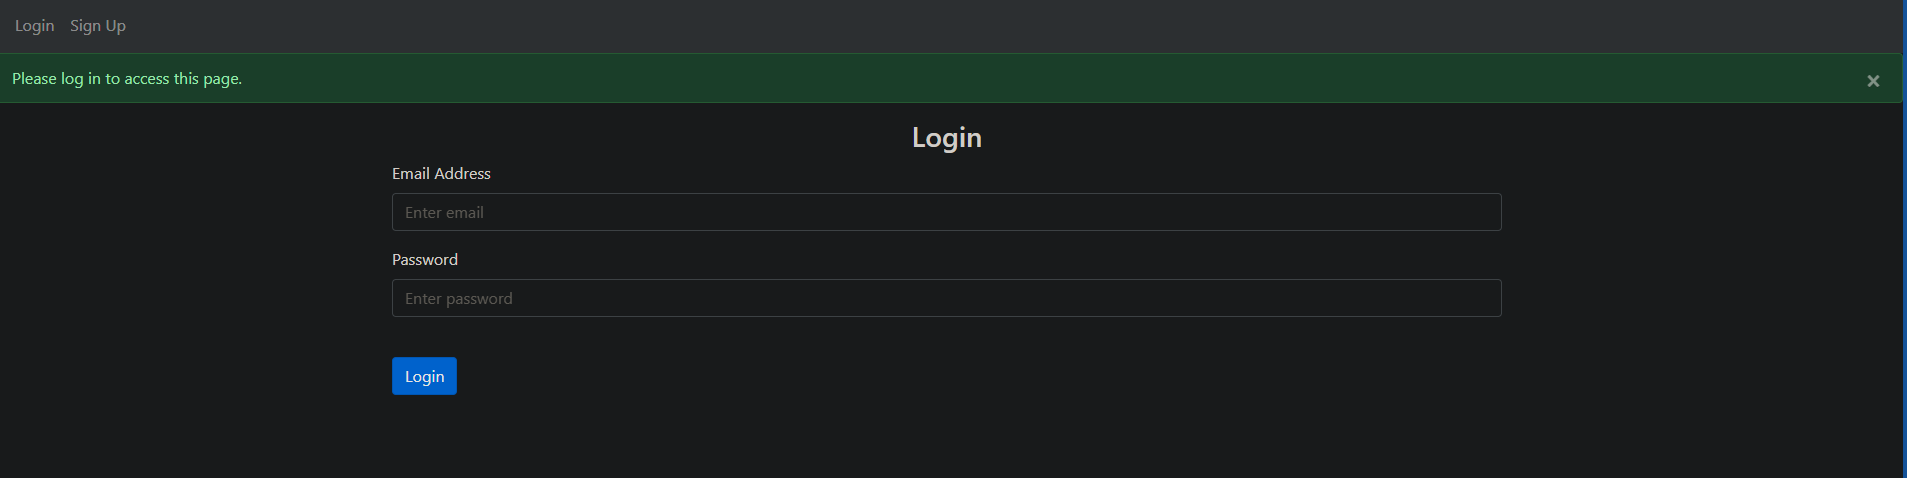
\includegraphics[width=16cm]{figs/login.png}
\caption{Página de login}
\label{fig:bookstack}
\end{center}
\end{figure}


Neste projeto foi usada como base de dados o SQLAlchemy do próprio Flask com a
seguinte estrura.
\begin{lstlisting}[language=csh, caption={Estrutura da base de dados}]
from . import db
from flask_login import UserMixin
from sqlalchemy.sql import func


class User(db.Model, UserMixin):
    id = db.Column(db.Integer, primary_key=True)
    email = db.Column(db.String(150), unique=True)
    password = db.Column(db.String(150))
\end{lstlisting}


Já no processo de autenticação os dados recebidos através do formulário da
página para serem verificados pelo seguinte código.

\begin{lstlisting}[language=csh, caption={Autenticação na página de login}]
@auth.route('/login', methods=['GET', 'POST'])
def login():
    if request.method == 'POST':
        email = request.form.get('email')
        password = request.form.get('password')

        user = User.query.filter_by(email=email).first()
        if user:
            if check_password_hash(user.password, password):
                flash('Login efetuado com sucesso!', category='success')
                login_user(user, remember=True)
                return redirect(url_for('views.home'))
            else:
                # messagem de erro opcional, o admin do sistema deve decidir se quer usar ou nao
                flash('Password incorreta', category='error') # pass incorreta
        else:
            flash('Credencias incorretas ou nao registadas', category='error') # email nao registado

    return render_template("login.html", user=current_user)
\end{lstlisting}

O \textit{email} e a hash (sha 256) da \textit{password} inseridos são verificados 
se existem na base de dados, se sim, a sessão é iniciada, caso contrário, o utilizador 
continua na página de \textit{login} e recebe (configuração de aviso de erro opcional
das linhas 13 e 16) um aviso do erro na página. \\




No caso da página de registo, poderá opcionalmente ser desativada, uma vez que 
apenas um numero mínimo
de utilizadores deverá ter acesso à funcionalidades de gestão de portas. \\

\begin{figure}[H]
\begin{center}
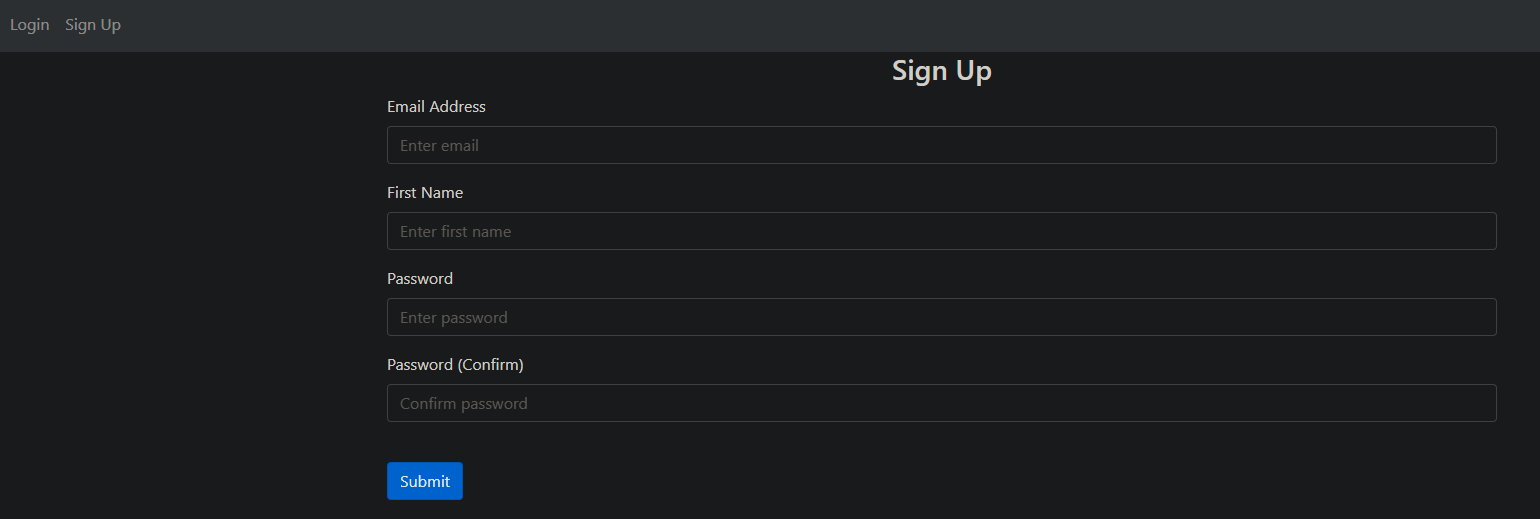
\includegraphics[width=16cm]{figs/registo.png}
\caption{Página de registo}
\label{fig:bookstack}
\end{center}
\end{figure}




\subsection{Página para fazer pedidos sobre portas}

\begin{figure}[H]
\begin{center}
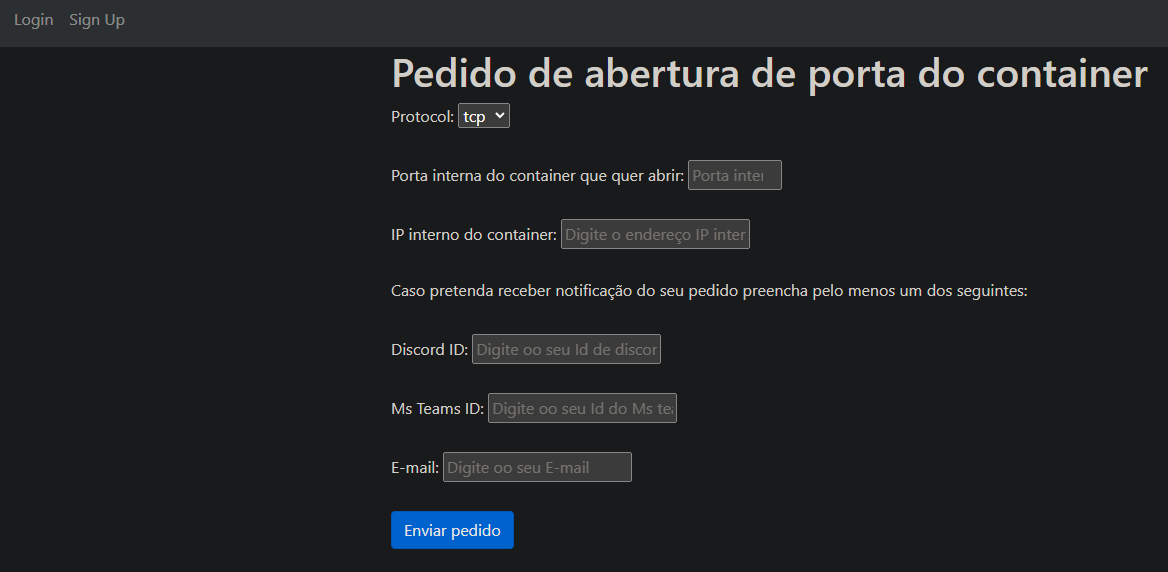
\includegraphics[width=16cm]{figs/pagina de pedidos2.png}
\caption{Página de de pedidos}
\label{fig:bookstack}
\end{center}
\end{figure}

Nesta pagina é possível inserir os dados para fazer o pedido ao administrador do
sitema para abrir uma determinada porta de modo dar aos utilizazdores da rede local
conectividade ao serviço aloja no \textit{container} na porta em questão. \\

Opcionalmente, é possivel inserir o ID do Discord, Microsoft Teams ou endereço E-mail
para receber notificação sobre o pedido.

\subsection{Página para criar a ligação NAT}

\begin{figure}[H]
\begin{center}
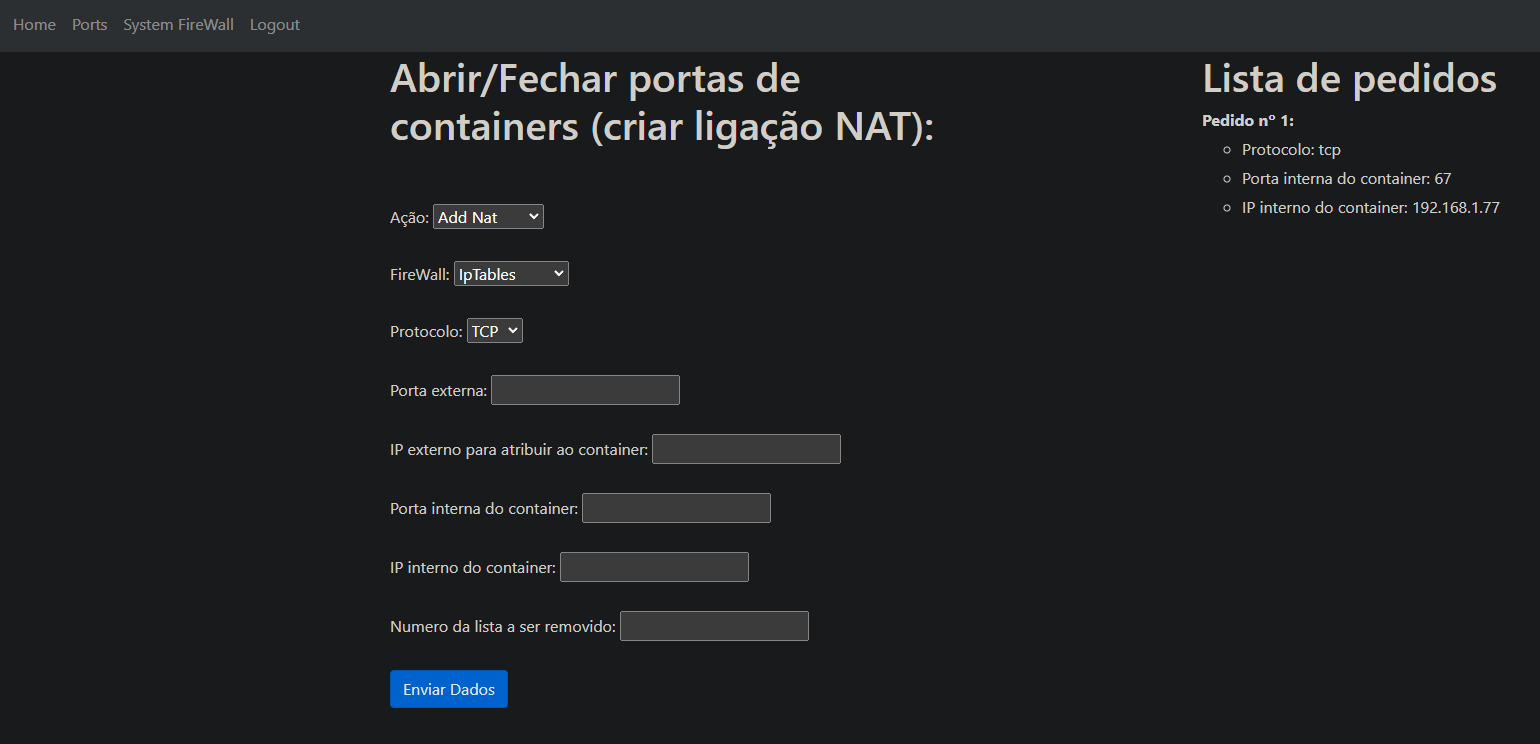
\includegraphics[width=16cm]{figs/criar nat 2.png}
\caption{Página para criar ligações NAT}
\label{fig:bookstack}
\end{center}
\end{figure}

O administrador do sistema ao inserir as suas credênciais tem acesso à página
para criar a ligação NAT. Nesta pagina é apresentado do lado direito
os pedidos pendentes, podendo associar uma porta juntamente com 
endereço IP do \textit{container} com uma porta e endereço IP exerternos. \\

O seguinte excerto de código mostra uma função em javascript onde é verificado
se todos os campos foram preenchidos e aplicada uma 
expressão regular para os campos de endreçoes IP, para garantir o formato correto.

\begin{lstlisting}[language=csh, caption={Código em javascript par verificar parâmetros da interface web}]
function validateForm() {
    const action = document.getElementById("action").value;
    const fw = document.getElementById("fw").value;
    const protocol = document.getElementById("protocol").value;
    const extPort = document.getElementById("ext_port").value;
    const extIp = document.getElementById("ext_ip").value;
    const intPort = document.getElementById("int_port").value;
    const intIp = document.getElementById("int_ip").value;

    if (!action || !fw || !protocol || !extPort || !extIp || !intPort || !intIp) {
        alert("Todos os campos devem ser preenchidos!");
        return false;
    }

    const ipPattern = /^(25[0-5]|2[0-4][0-9]|1[0-9]{2}|[1-9]?[0-9])(\.(25[0-5]|2[0-4][0-9]|1[0-9]{2}|[1-9]?[0-9])){3}$/;
    if (!ipPattern.test(intIp)) {
        alert("Por favor, insira um endereco IP valido.");
        return false;
    }

    if (!ipPattern.test(extIp)) {
        alert("Por favor, insira um endereco IP valido.");
        return false;
    }

    return true;
}
\end{lstlisting}




O seguinte excerto de código python mostra o que acontece quando os dados são enviados.
\begin{lstlisting}[language=csh, caption={Código em python da interface web}]
@views.route('/nat', methods=['GET', 'POST']) 
def nat():

    if request.method == 'POST':
            
        action = request.form.get('action')
        fw = request.form.get('fw')
        protocol= request.form.get('protocol')
        ext_port = request.form.get('ext_port')
        ext_ip = request.form.get('ext_ip')
        int_port = request.form.get('int_port')
        int_ip = request.form.get('int_ip')
        chave = request.form.get('key_to_remove')

        print(action)
        print(fw)
        print(protocol)
        print(ext_port)
        print(ext_ip)
        print(int_port)
        print(int_ip)

        # descomentar esta linha para enviar dados par o port controller
        #hostnat(action, fw, protocol, ext_port, ext_ip, int_ip, int_port)

        try:
            notificar(int(chave))
            remove_item(int(chave))
        except:
            print("Erro nao foi recebido nenhum valor para remover da lista de pedidos")

            
        return redirect(url_for('views.nat', dicionario=pedidos , user=current_user))

    return render_template('nat.html', dicionario=pedidos , user=current_user)
\end{lstlisting}

É possivel reparar que este código recebe os dados do formulário preenchido da página HTML
para, de seguida, na linha 17 serem enviadas notificações para os utilizadores que inseriram
pelo menos um ID (Discord ou Microsoft Teams).

Na linha 18 é removido o pedido, referente aos dados preenchidos, do dicionário no qual estava guardado.

Na linha 31 é chamada a função "hostnat" do ficheiro "unisSocketConn.py" onde são passados 
os valores do formulário para serem enviados para o "Port Controller" e por sua vez execudada
a ação de acordo com esses mesmos dados.

Por fim na linha 32, a página é atualizada e juntamente com o contéuda do dicionário "pedidos".





\title*{\textbf{Página para abrir/fechar portas do sistema host}}

\begin{figure}[H]
\begin{center}
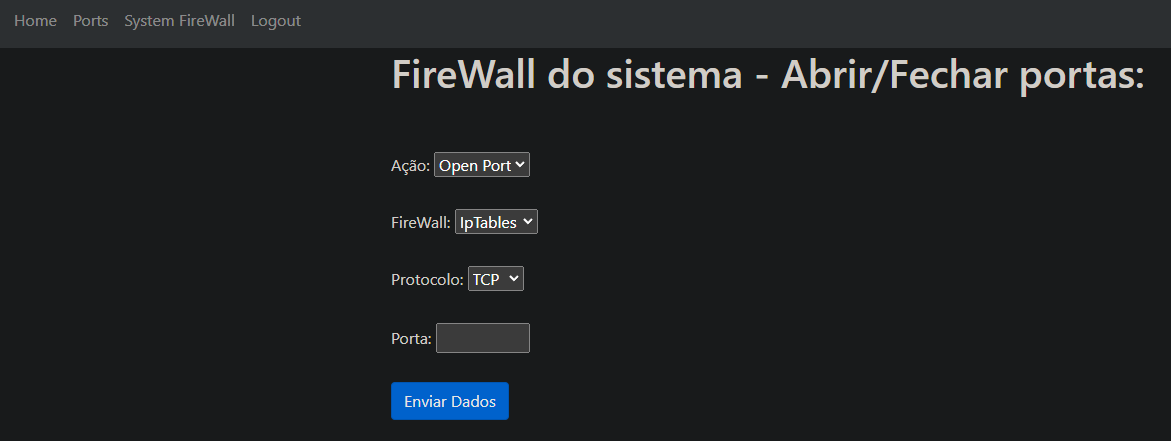
\includegraphics[width=16cm]{figs/sysfirewall.png}
\caption{Página de da firewall do sistema}
\label{fig:bookstack}
\end{center}
\end{figure}

É também possível abrir e fechar portas da \textit{firewall} (Iptables) 
do sistema \textit{host}.








%================================================================================

\section{Sistema de notificações}

Para notificar os utilizadores que fizeram pedidos para abrir uma determinada
porta podem opcionalmente receber uma notificação quando o seu pedido é aceite 
através do Discord, Microsoft Teams ou E-mail.

\subsection{Discord}

Para a implemetação de enviar notificações para um utilizador no Discord,
não foi criado um "\textit{Bot}", mas sim uma conta normal, uma vez que o objetivo é apenas
enviar mensagem direta para um utilizador e não gerir um servidor.

\begin{lstlisting}[language=csh, caption={Envio de notificação via Discord}]
import os
from dotenv import load_dotenv, dotenv_values
import requests

#load from .env
load_dotenv('.env')
key: str = os.getenv('KEY')


def createDm(user_id):
    payload = {
        'recipient_id': user_id
    }
    
    header = {
        'Content-Type': 'application/json',
        'authorization': key
    }

    url = "https://discord.com/api/v9/users/@me/channels"
    
    r = requests.post(url, json=payload, headers=header)
    print(r.status_code)
    #print(r.json())

    channel_id = r.json()['id']
    
    return channel_id

def send_dm(user_id):

channel_id = createDm(user_id)

url = f"https://discord.com/api/v9/channels/{channel_id}/messages"


header = {  
    'authorization': key
}

payload = {
    'content': "O seu pedido foi conluido"
}


r = requests.post(url, data=payload, headers=header)
print(r.status_code)
\end{lstlisting}

Neste excerto de código é carregado de um ficheiro .env o token da conta, usado para
a autenticação das solicitações feitas ao longo do procedimento.

A função "createDm" (linha 10) envia uma solicitação POST apenas para criar o canal de texto
com o utilizador e enviar o ID desse mesmo canal para a função "send\_dm".

Para de seguida, a função "send\_dm" (linha 30) enviar a mensagem (solicitação POST) para 
o canal. Fazendo assim, que o utilizador receba uma mensagem direta.

Sendo assim, é apenas chamar a função "send\_dm" e passar-lhe o argumento do ID do utilizador. \\



%======================================================================================

\subsection{Microsoft Teams}

Para enviar notificações para um utilizador via Miscrosoft Teams, ao contrário do Discord,
é necessário criar um \textit{Bot} com um \href{https://learn.microsoft.com/en-us/azure/bot-service/bot-service-overview?view=azure-bot-service-4.0}{\textit{Framework}}
fornecido pela Microsoft. \\



\title*{\textbf{Registo do Bot no Azure}}

Para poder criar um Bot para o Microsoft Teams é necessário registar o mesmo 
no "Azure Bot" do \textit{Marketplace} do Azure.

\begin{figure}[H]
\begin{center}
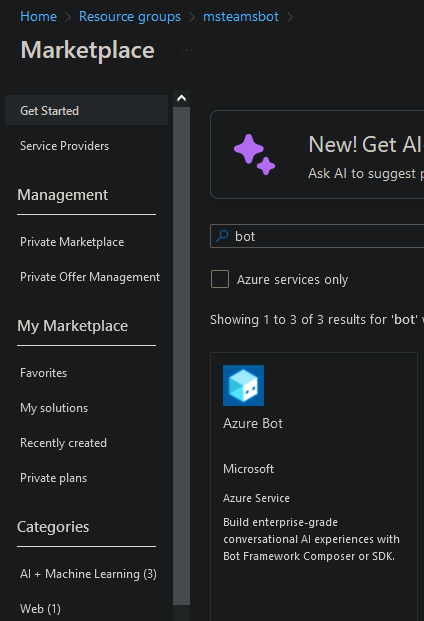
\includegraphics[width=14cm]{figs/marketplace azure bot.png}
\caption{Azure Bot do Marketplace do Azure}
\label{fig:bookstack}
\end{center}
\end{figure}

De seguida é apenas necessário preencher os parâmetros necessários de modo a obter
a seguinte configuração.

\begin{figure}[H]
\begin{center}
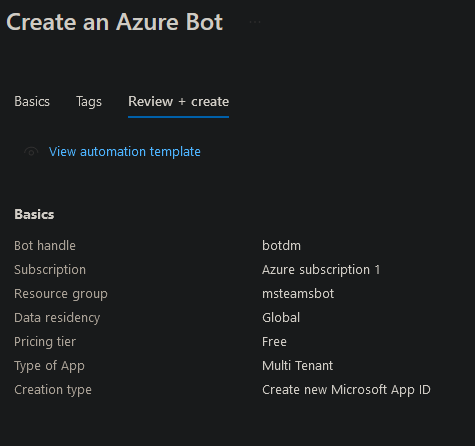
\includegraphics[width=14cm]{figs/detalhes do bot.png}
\caption{Detalhes do registo do BOT}
\label{fig:bookstack}
\end{center}
\end{figure}


Contudo, durante o passo de registo do BOT ocorreu o seguinte erro que impossibilitou
a contiinuação do processo. O erro deve-se ao facto da conta utilizada associada à 
instituição de ensino não ter as permissões necessárias.

\begin{figure}[H]
\begin{center}

\includegraphics[width=10cm]{figs/erro bot azure.png}
\caption{Erro do Azure no registo do BOT}
\label{fig:bookstack}
\end{center}
\end{figure}



\title*{\textbf{Funcionamento do código (Teórico)}}

Durante o processo de desenvolvimento de código foi consultado o \href{https://github.com/microsoft/BotBuilder-Samples/tree/main/samples/python/02.echo-bot}{Github da Microsoft}
com exemplos de código para Bots, no caso, para a linguagem Python.

Para garatir o funcionamento do bot é necessário instalar as seguintes bibliotecas:
\begin{itemize}
    \item botbuilder-core
    \item botbuilder-schema
    \item botbuilder-integration-aiohttp
    \item aiohttp
\end{itemize}


O seguinte excerto de código mostra o funcionamento do envio de mensagens via Microsoft Teams.

\begin{lstlisting}[language=csh, caption={Envio de notificação via Microsoft Teams}]
from aiohttp import web
from botbuilder.core import BotFrameworkAdapter, BotFrameworkAdapterSettings, TurnContext
from botbuilder.schema import Activity, ActivityTypes, ConversationReference

import os
import asyncio

app_id = os.getenv("MICROSOFT_APP_ID", "my-app-id")
app_password = os.getenv("MICROSOFT_APP_PASSWORD", "my-app-password")
settings = BotFrameworkAdapterSettings(app_id, app_password)
adapter = BotFrameworkAdapter(settings)


conversation_references = {}

async def send_proactive_message(conversation_reference: ConversationReference, message: str):
    async def aux(turn_context: TurnContext):
        await turn_context.send_activity(Activity(type=ActivityTypes.message, text=message))

    await adapter.continue_conversation(conversation_reference, aux, app_id)

async def messages(req: web.Request) -> web.Response:
    body = await req.json()
    activity = Activity().deserialize(body)

    if activity.type == ActivityTypes.message and "Ola" in activity.text:
        # Criar a referencia da conversa
        conversation_reference = TurnContext.get_conversation_reference(activity)
        user_id = activity.from_property.id
        conversation_references[user_id] = conversation_reference

        # Enviar mensagem para o utilizador
        asyncio.create_task(send_proactive_message(conversation_reference, "Ola! o seu pedido foi concluido."))

    return web.Response(text="OK")


async def send_message_to_user(req: web.Request) -> web.Response:
data = await req.json()
user_id = data.get("user_id")
message = data.get("message")

if user_id in conversation_references:
    conversation_reference = conversation_references[user_id]
    await send_proactive_message(conversation_reference, message)
    return web.Response(text="Mensagem enviada.")
else:
    return web.Response(status=404, text="Utilizador nao encontrado.")



app = web.Application()
app.router.add_post("/api/messages", messages)
app.router.add_post("/api/send-message", send_message_to_user)

if __name__ == "__main__":
    port = int(os.environ.get('PORT', 3900))
    web.run_app(app, port=port)

\end{lstlisting}

O código apresentado deve estar a ser executado num servidor que seja acessivel pela
aplicação da interface \textit{web} para apartir desta, ser enviada uma solicitação POST
para o caminho "/api/send-message". \\

O seguinte excerto de código mostra a função que é chamada apartir da aplicação
da interface \textit{web} para enviar notificação para os utilizadores.
\begin{lstlisting}[language=csh, caption={Solicitação para enviar mensagem}]
import requests

def SendeDm(user_id):

    payload = {
        "user_id": user_id,
        "message": "O seu pedido foi conluido"
    }
    
    header = {
        'Content-Type': 'application/json'
    }

    url = "http://localhost:3900/api/send-message"
    
    r = requests.post(url, data=payload, headers=header)
    print(r.status_code)
\end{lstlisting}

Esta funcionalidae de notificações pode ser testada também com o seguinte comando.
\begin{lstlisting}[language=csh, caption={Teste de notificação via Microsoft Teams}]
    curl -X POST -H "Content-Type: application/json" -d '{"user_id": "USER_ID", "message": "conteudo da mensagem direta"}' http://localhost:3978/api/send-message
\end{lstlisting}


\subsection{Notificação via E-mail}

O seguinte código mostra a função responsável por enviar notificações via E-mail.

\begin{lstlisting}[language=csh, caption={Teste de notificação via Microsoft Teams}]
import smtplib
import os
from dotenv import load_dotenv, dotenv_values


#load from .env
load_dotenv('.env')
password: str = os.getenv('PASSWORD')


def Send_email(email):
    
    sender_email = "a036785@ipmaia.pt"

    
    
    receiver_email = email
    
    subject = "Pedido de porta"
    mensagem = "O seu pedido foi aceite"
    
    text = f"Subject: {subject} \n\n{mensagem}"
    
    #server = smtplib.SMTP("smtp.gmail.com", 587)
    server = smtplib.SMTP("smtp-mail.outlook.com", 587)
    server.starttls()
    
    server.login(sender_email, password)
    
    server.sendmail(sender_email, receiver_email, text)
    
        
\end{lstlisting}

Neste excerto de código é apenas necessário fazer a importação à biblioteca core
"smtplib". 
Para evitar expor a palavra passe do email que envia a mensagem no código a mesma 
é carregada a partir de um ficheiro .env .





\section*{Sumário}

Será configurado o ambiente de testes em Alpine Linux, onde serão realizados testes
de \textit{firewall} e LXC/LXD, através de linha de comandos, com o objetivo de entender 
o funcionamentos destas ferramentas, para de seguida, poder implementar, de forma mais eficaz,
ações relacionadas a estas, mas através de código (no "Port Controller"). São também 
explicadas as implementações da REST API, Interface web, unix socket e sistemas de notificações.

%Ver o \nameref{sec:intro_summary} página \pageref{sec:intro_summary} para perceber como utilizar esta secção.








% PT: opcional
\chapter{Desvios de Procedimento}
\label{cap:detour}

%Este capítulo é opcional e o seu objectivo é descrever os pontos de discordância

Durante o desenvolvimento do projeto o único contratempo que ocorreu foi o facto da conta
do Azure não possuir permissões para registar o BOT, que por consequênte impediu a realização
de testes com o mesmo.



% PT: opcional
\chapter{Discussão de resultados}
\label{cap:results}
%Este capítulo é opcional e pode ser omitido, mas destina-se a responder às seguintes questões:
%\begin{enumerate}
%    \item Que resultados foram obtidos?
%    \item O que é que se conseguiu com isso?
%\end{enumerate}

Neste projeto, as tarefas principais (Implementação de um daemon de gestão de portas
e respetctivo interface \textit{web} e suporte a notificações), inicialmente 
apresentadas na proposta foram concluídas com sucesso.

No caso do daemon, foi implementado com multi \textit{threading} e com interage com
o LXC através da API do LXD de modo a ter capacidade de executar multiplas tarefass com a melhor
\textit{performance}.

No sistema de notificações, existe a possiblidade de usar Discord, E-mail e teoricamente Microsoft Teams.

Adicionalmente, pode ser usada a REST API para interagir com daemon ("Port Controler")
através da linha de comandos, caso se pretenda assim fazer.

De modo geral, foi concebido diversos componentes funcionais que podem ser integrados no
devlab(plataforma forge) do IPMAIA/UMAIA.

% PT: opcional
\chapter{Trabalho futuro}
\label{cap:future}

Este capítulo é opcional, devendo ser usado apenas se pretender listar  trabalho futuro ou caminhos possíveis para trabalho futuro de continuação deste projecto.


\chapter{Conclusões e reflexão crítica}
\label{chap:conclusions}

%Neste capítulo deve apresentar as suas conclusões e realizar uma reflexão crítica do trabalho desenvolvido e da sua participação na empresa.

O desenvolvimento deste projeto foi extremamente intressante de realizar, uma vez, que
existe a possibilidade de o mesmo ser integrado no DevLab. Para além disso, o mesmo foi 
concebido com um conjunto de tecnologias, desde as linguagens de programação, aos protocolos, 
sistemas operativos, que com a sua junção se tornou num desafio capaz de testar e aumentar
os conhecimentos do autor do projeto.






\addcontentsline{toc}{chapter}{Referências}

\printbibliography[title={Referências\label{chapter:refs}}]

\label{lastpage1}

\clearpage

\pagenumbering{arabic}
\renewcommand*{\thepage}{A\arabic{page}}
\appendix
%\begin{appendices}

\chapter{Especificação de requisitos simplificada}
\label{chap:za}

Este é um exemplo de um anexo do documento. É frequente ser necessário listar um conjunto de requisitos que regem o planeamento do projecto. Se assim for, o ideal será colocá-los aqui.
\chapter{Questionários}
\label{chap:zb}

É muito frequente ser necessário realizar questionários para validar a ideia que está a ser trabalhada, de vários pontos de vista:

\begin{enumerate}
    \item do ponto de vista de como é que o público alvo encara uma necessidade que esta ideia pode suprimir;
    \item do ponto de vista de como é que o público alvo reagiu à possibilidade desta ideia ser posta em prática;
    \item do pontos de vista de como é que o público alvo reagiu à interacção com uma implementação da ideia.
\end{enumerate}

Caso tenha procedido à construção de questionários, use este anexo para listar as perguntas efectuadas, bem como os resultados obtidos. Caso tenha realizado vários questionários diferentes (como os listados na enumeração anterior, por exemplo), separe-os por secções.
%\end{appendices}
\label{lastpage2}
\end{document}